\documentclass{article}
\usepackage{graphicx} % Required for inserting images
\usepackage{amsmath}
\usepackage{amsfonts}
\usepackage{float}
\usepackage{xcolor}

\definecolor{light-gray}{gray}{0.95}
\newcommand{\code}[1]{\colorbox{light-gray}{\texttt{#1}}}

\title{Applied Statistics - Exam Notes}

\date{Spring 2024}

\begin{document}

\maketitle

\tableofcontents

\pagebreak

\section{Introduction}

\subsection{Population Data}

\begin{itemize}
    \item Is the data for an \textbf{entire} group, class, or type of people or objects, defined by the researcher
    \item Population can be quite large, rarely can we collect data on all members of population; time and expense
    \item But, we still need to be able to make conclusions about the entire population
    \item When we do collect data about every member, it's called a census
\end{itemize}

\subsection{Sample Data}

\begin{itemize}
    \item When we need to make conclusions or estimates about an entire population, we almost always use a sample(s) from our population of interest
    \item A small but well-chosen sample can accurately reflect the characteristics of the entire population from which it is chosen, \textbf{it should be representative of the population from which it is drawn}
    \item All elements in a sample must also by definition be part of the population it is defined
    \item In almost all cases, samples from the same population should be independent from each other
    \item In many cases, the sample is chosen randomly from the population (random sample); but there are other methods
\end{itemize}

\subsection{Population vs Sample}

\begin{tabular}{|l|c|c|}
\hline
 & \textbf{Population} & \textbf{Sample} \\
\hline
\textbf{Measurement} & Parameter & Statistic \\
\textbf{Mean} & $\mu$ & $\bar{x}$ \\
\textbf{Variance} & $\sigma^2$ & $S^2$ \\
\textbf{Standard Deviation} & $\sigma$ & $S$ \\
\hline
\end{tabular}

\begin{itemize}
    \item You will often see two versions of formulas; one for a population and one for a sample
    \item A sample is always an approximation of a population, therefore: sample data always have error bars built into them; uncertainty
\end{itemize}

For example, population standard deviation vs sample standard deviation

\begin{align*}
    \sigma=\sqrt{\frac{\sum{(X-\mu)}^2}{n}}, s= \sqrt{\frac{\sum{(x-\bar{x})}^2}{n-1}}
\end{align*}

Where $n-1$ indicates one less degree of freedom as we are estimating one parameter in the population.

\subsection{Linear Transformation}

Linear transformation of mean and standard deviation:

\begin{itemize}
    \item Let $\bar{y}$ and $s$ be the sample mean and standard deviation from observations $y_1,y_2,\dots,y_n$ 
    \item Let $z_i=c \cdot y_i + b$ be a linear transformation of the $y$'s with constants $b$ and $c$
    \item Then, $\bar{x}=c \cdot \bar{y} + b$
    \item $s_z= |c| \cdot s_y$
\end{itemize}

\section{Descriptive Statistics}

\subsection{Categorical and Quantitative Data}

\begin{itemize}
    \item Categorical data use labels, names, or other descriptions to identify \ {exclusive} categories or types of things
        \begin{itemize}
            \item $\text{Relative frequency of a class} = \frac{\text{Frequency of the class}}{n}$
            \item Frequencies/relative frequencies of categories can be plotted as bar charts, or represented as tables
        \end{itemize}
    \item Quantitative data are numerical values that represent frequency, measurement, etc.
        \begin{itemize}
            \item Quantitative data can be split into bins, with each bin having a range (i.e. 0-9, 10-19, 20+). There must be no overlap
            \item Too few or too many bins may not show the underlying shape/distribution
            \item Bins can be plotted onto a \textbf{histogram}, like a bar chart (but without gaps), but for frequencies/relative frequencies of bins.
            \item Histograms can have a left/right skew. The tail is thinner on the skew side. So, left skew = thin tail on left side, clumped up on right side
            \item Other shapes:
            \begin{itemize}
                \item \textbf{Symmetric}: Same on the left/right
                \item \textbf{Bimodal}: Two distinct peaks
                \item \textbf{Uniform}: Same height for each bin
                \item \textbf{No pattern}: Seemingly random
            \end{itemize}
        \end{itemize}
\end{itemize}

\subsection{Cross Tabulation}

\begin{itemize}
    \item Cross tabulation is a table summary for two variables
    \item Used to show relationship between two variables
    \item Variables can be categorical or quantitative (in bins)
    \item Cross tabs have total cells for each column and row, and grand total in lower-right corner
\end{itemize}

\subsection{Mean, Median, and Mode}

\begin{itemize}
    \item \textbf{Mean}: The average of all observations in the data, so $\frac{\sum{x}}{n}$
    \item \textbf{Median}: The middle observation of the data, after sorting from smallest to largest. If $n$ is even, the median is the mean of the two middle values
    \item \textbf{Mode}: The observation that occurs the most often in the data. A dataset can have one, multiple, or no modes
    \item \textbf{Trimmed Mean}: We sort the data, then remove the same number/percentage of observations from both ends; then calculate mean from remaining observations
\end{itemize}

\subsection{Grouped Frequencies}

\begin{itemize}
    \item \textbf{Grouped Frequency Mean}: A very close approximation of the sample mean; the higher the count in each bin and the narrower the bin range, the better it will be. For each bin:
    \begin{enumerate}
        \item Find midpoint $\text{m} = \frac{\text{upper bound} + \text{lower bound}}{2}$ 
        \item Multiply each midpoint by it's frequency
        \item Sum all the values from step 2
    \end{enumerate}
    \item \textbf{Grouped Frequency Std Deviation}: $s_x = \sqrt{\frac{\sum_{i=0}^j{(m_i-\bar{x})^2f_i}}{n-1}}$, for $j$ bins, and $n$ sample size. As always, $s_x^2$ is the grouped frequency variance.
\end{itemize}

\subsection{Percentiles, Quartiles, Quintiles, and Deciles}

\begin{itemize}
    \item All variations of the same thing (percentiles)
    \item Locate an observation's position in a sorted dataset; they don't have to be an actual value in the dataset
    \item Percentiles represent the number of values out of the total that are at or below that percentile
    \item Quartiles split the data into 4 parts, quintiles 5, deciles 10
    \item 50th percentile/2nd quartile/5th decile = Median
    \item \textbf{Location Formula}: $L_p = \frac{p}{100}(n+1)$, where $L$ is a location in the sorted data, $p$ is the percentile, $n$ is the number of observations in the data
    \item \textbf{IRQ} is the range from quartile 1 to quartile 3, so percentile 25 to 75
\end{itemize}

\subsection{Box Plots}

\begin{itemize}
    \item Easy way to identify outliers, easy to interpret
    \item Makes comparing characteristics of data between categories very easy
    \item As a rule of thumb, any value more than 1.5 IQR from Q1/Q3 is an outlier. Whiskers go up to there, or when closer, the min/max observations
\end{itemize}

\begin{figure}
    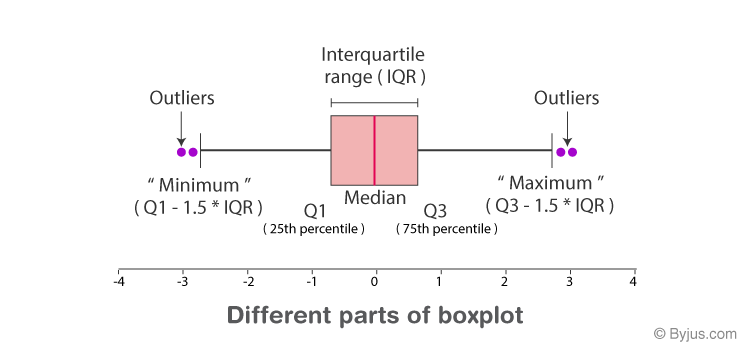
\includegraphics[width=1.0\linewidth]{Box-Plot-and-Whisker-Plot.png}
\end{figure}

\subsection{Variance, Standard Deviation and Z-scores}

\begin{itemize}
    \item Variance is $\sigma^2$ "sigma squared" (sample)
    \item Standard Deviation is $\sigma$ "sigma" (sample)
    \item $\sigma = \sqrt{\frac{\sum_{i=0}^{n}{(x_i-\bar{x})^2}}{n-1}}$
\end{itemize}

\begin{itemize}
    \item Z-scores ignore measurement units, measure distance from mean in amount of standard deviations
    \item Mean has a Z-score of zero
    \item $Z = \frac{\text{data point} - \text{mean value}}{\text{standard deviation}}=\frac{X-\bar{X}}{s}=\frac{x-\mu}{\sigma}$
\end{itemize}

\subsection{Bivariate Relationships}

\subsubsection{Covariance}

\begin{itemize}
    \item Covariance - co-vary - how they change together
    \item Used to analyze the linear relationship between two variables - how do they behave as a pair?
    \item A positive value indicates a direct or increasing linear relationship, a negative value indicates a decreasing relationship
    \item The covariance indicates \textbf{direction, not strength}. Correlation is for strength
    \item When there's no pattern, the covariance is near 0
    \item \textbf{Sample Covariance}: $s_{xy}=\frac{\sum_{i=0}^n{(x_i-\bar{x})(y_i-\bar{y})}}{n-1}$
    \item \textbf{Population Covariance}: $\sigma_{xy}=\frac{\sum_{i=0}^N{(x_i-\mu_x)(y_i-\mu_y)}}{N}$
\end{itemize}

\subsubsection{Covariance Matrix}

\begin{itemize}
    \item Essentially cross tabulation, but instead of frequencies, it shows covariances between each r/c pair
    \item The diagonal just shows the variance
    \item Top-right and bottom-left triangles are the same
\end{itemize}

\begin{figure}[H]
    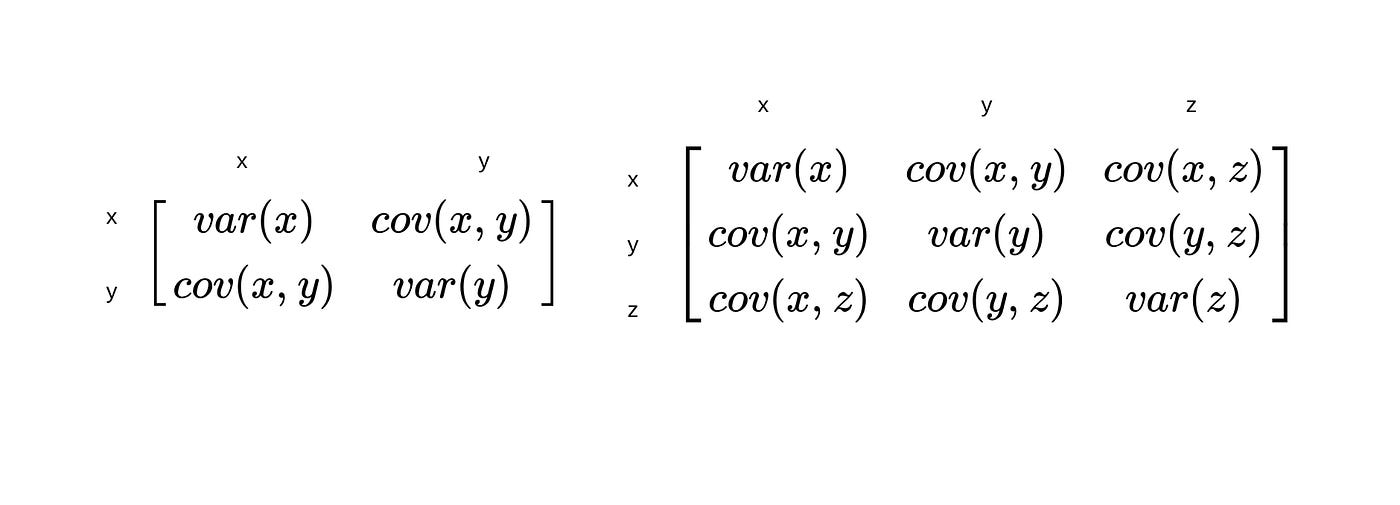
\includegraphics[width=1\linewidth]{Covariance-Matrix.jpg}
\end{figure}

\subsubsection{Correlation}

\begin{itemize}
    \item Correlation provides \textbf{direction and strength} of the relationship between two variables
    \item Always between $-1$ and $+1$; scale independent of variables' scales
    \item Only applicable to linear relationships
    \item Correlation strength does not necessarily mean the correlation is statistically significant; related to sample size
    \item $r$ is called the Pearson correlation coefficient
    \item $r=\frac{\text{Cov}(x,y)}{s_xs_y}$
\end{itemize}

\section{Permutations and Combinations}

\subsection{Permutations}

\textbf{Permutations - Order matters}: The number of different ways that a certain number of objects $r$ can be \textbf{arranged in order} from a larger number of objects $n$

 \begin{itemize}
    \item If there are $n$ objects, how many different ways can we make ordered lists of size $r$
    \item Written as $_nP_r$ or $P(n,r)$
    \item $_nP_r=\frac{n!}{(n-r)!}$
    \item \textbf{TI84}: \code{MATH -> PROB -> nPr}
\end{itemize}

\subsection{Combinations}

\textbf{Combinations - Order doesn't matter}: The number of different ways that a certain number of objects $r$ (as a group) can be selected from a larger number of objects $n$

\begin{itemize}
    \item Often said as "n choose r"
    \item If there are $n$ objects, how many different ways can we select \textbf{groups or sets} of size $r$
    \item Written as $_nC_r$ or $C(n,r)$
    \item $_nC_r=\binom{n}{r}=\frac{n!}{r!(n-r)!}$
    \item \textbf{TI84}: \code{MATH -> PROB -> nCr}
    \item It can be useful to calculate $\sum_{r=0}^{n}{_nC_r}$, then take any other combinations as fractions of this sum; this gives you the probability of getting those combinations out of all possible ones
\end{itemize}

\section{Discrete Probability Distributions}

\subsection{Random Variable}

\begin{itemize}
    \item A random variable (r.v.) is a variable that takes on numerical values as a result of random experiments or measurement; associates a numerical value with each possible outcome
    \item Usually denoted by a capital letter like $X$ or $Y$
    \item A discrete r.v. has a finite number or an infinite sequence of values, unlike a continuous r.v.  which has an infinite number of outcomes
    \item The probability distribution for a r.v. $X$ describes how probabilities are assigned to each outcome
    \item For any outcome, $0 \leq P(x) \leq 1$, and sum of all r.v. outcome probabilities must equal 1 ($\sum_{i=0}^{n}(P(x_i))=1$)
    \item \textit{Example}: Uniform distribution, each outcome equally as likely to occur with probability $1/n$ where $n$ is number of outcomes
\end{itemize}

\subsubsection{Expected value}

\begin{itemize}
    \item The expected value is the mean of a r.v.; the average expected outcome. It does not have to be a value the discrete r.v. can assume
    \item $E(x)=\mu=\sum_{i=0}^{n}(x_i \cdot P(x_i))$
\end{itemize}

\subsubsection{Variance}

\begin{itemize}
    \item Variance and standard deviation is a measure of how disperesed the r.v. is relative to it's mean
    \item $\text{Var}(x)=\sigma^2=\sum_{i=0}^{n}((x_i - \mu)^2 \cdot P(x_i))$
    \item Standard deviation $\sigma=\sqrt{\text{Var}(x)}$
\end{itemize}

\subsection{Binomial Distribution}

\begin{itemize}
    \item A binomial experiment has:
    \begin{itemize}
        \item A sequence of $n$ trials
        \item Only two exclusive outcomes are possible in each trial. One outcome is called a "success" and the other a "failure"
        \item The probability of a success is denoted by $p$, does not change from trial to trial. The probability of failure is $1-p$ and is also fixed
        \item The trials are independent; the outcome of previous trials doesn't influence future trials
    \end{itemize}
    \item $_nC_x \cdot p^x \cdot (1-p)^{n-x}$, where $n$ is number of trials, $x$ is number of successes, $p$ is the probability of success in any trial
    \item \textbf{TI84}:
    \begin{itemize}
        \item Find $P(X=x)$: \code{DISTR -> binompdf}
        \item Find $P(X \leq x)$: \code{DISTR -> binomcdf}
        \item Find smallest $x$ for which $P(X \leq x) \geq c$ \code{DISTR -> invBinom} \code{area:c}
    \end{itemize}
\end{itemize}

\subsubsection{Binomial Mean and Standard Deviation}

\begin{itemize}
    \item $\mu=n \cdot p$
    \item $\sigma = \sqrt{n \cdot p \cdot (1-p)}$
\end{itemize}

\subsubsection{Proportions}

\begin{itemize}
    \item See slides 10.2 for info about proportions in the context of binomal distributions/binary count data
    \item For the difference of proportions, CI is: $\hat{p_1}-\hat{p_2} \pm z_{\alpha/2} \sqrt{\frac{\hat{p_1}(1-\hat{p_1})}{n_1}+\frac{\hat{p_2}(1-\hat{p_2})}{n_2}}$
    \item CLT gives that the sample proportions are asymptotically normal:
    \begin{itemize}
        \item $\hat{p_1} \approx N(p_1,p_1(1-p_1)/n_1)$
        \item $\hat{p_2} \approx N(p_2,p_2(1-p_2)/n_2)$
    \end{itemize}
\end{itemize}

\subsection{Multinomial Distribution}

\begin{itemize}
    \item If the vector of counts $(Y_1,\dots,Y_c)$ has a multinomial distribution, then:
    \begin{itemize}
        \item $p(y_1,\dots,y_c)=\frac{n!}{y_1! \cdot \dots \cdot y_c!} \prod_{j=1}^c p_j^{y_j}$
        \item Where $y_1+\dots+y_c=n$ and $p_1+\dots+p_c=1$
    \end{itemize}
    \item For two categories, $(Y_1, Y_2)$, we typically just think of it as binomial with one category representing a pass and the other a fail
    \item The outcome $Z_i$ of the $i$'th trial can be represented through a vector $Z_i=(Z_{i1},\dots,Z_{ic})$ with $Z_{ij}=$
    \begin{itemize}
        \item $=1$ if outcome in category $j$
        \item $=0$ otherwise
    \end{itemize}
    \item The random variable $n_j$ counts the number of times a trial leads to category $j$, i.e. $Y_j=\sum_{i=1}^n Z_{ij}$
    \item $E(Y_j)=\sum_{i=1}^n P(Z_{ij}=1)=n\hat{p_j}$
    \item \textbf{Properties}:
    \begin{itemize}
        \item The sum of multinomially distributed variables is again multinomial, if the probability vectors are identical - we simply have more independent identical trials
        \item If categories are merged, the new vector of counts also has a multinomial distribution - just add the probabilities for the merged categories
        \item The count for a single category is binomial - merge all other categories into one
    \end{itemize}
    \item The MLE for the multinomial proportions $p_1,...,p_c$ is the proportions of samples in each category: $\hat{p_j}=\frac{n_j}{n}$
    \item See Week 11.1 slides for Chi-Squared test info/example for multinomial distributions
    \item See Week 11.2 slides for contingency tables
\end{itemize}

\section{Continuous Probability Distributions}

\begin{itemize}
    \item In a continuous probability distribution, the probability of any specific outcome is 0
    \item Instead, you need to calculate the probability for an interval
\end{itemize} 

\subsection{Uniform Continuous Distribution}

\begin{itemize}
    \item $f(x)=\frac{1}{(b-a)}$, where $a$ is the min, and $b$ is the max
    \item $\text{E}(X)=\frac{a+b}{2}$
    \item $\text{Var}(X)=\sigma^2=\frac{(b-a)^2}{12}$
    \item $\text{Std}(X)=\sigma=\frac{b-a}{\sqrt{12}}$
\end{itemize}

\subsection{Normal Distribution}

\begin{itemize}
    \item Symmetric around mean
    \item Top/center of curve is $u$, median, and mode
    \item Smaller $\mu$ makes curve narrower, bigger $\mu$ will make it wider
    \item Area under curve always 1
    \item Standard normal curve - \textbf{Z Distribution} - is normal with $\mu=0$ and $\sigma=1$
    \item $z$ is a measure of how many $\sigma$ away from $\mu$
    \item $68.28\%$ within $1\sigma$ of $\mu$, $94.44\%$ within $2\sigma$, and $99.72\%$ within $3\sigma$
    \item $f(x)=\frac{1}{\sigma \sqrt{2\pi}}e^{-\frac{1}{2}(\frac{x-\mu}{\sigma})^2}$
    \item \textbf{TI84}:
    \begin{itemize}
        \item Find $f(x)$: \code{DISTR -> normalpdf}
        \item Find $P(a\leq X\leq b)$: \code{DISTR -> normalcdf} \code{lower:a upper:b}
        \item Find z-score for given probability $p$: \code{DISTR -> invNorm} \code{area:p}; for \code{TAIL}:
        \begin{itemize}
            \item \code{LEFT} returns z-score to the left of which the area is equal to $p$
            \item \code{CENTER} returns $\pm$z-score between which the area is equal to $p$
            \item \code{RIGHT} returns z-score to the right of which the area is equal to $p$
        \end{itemize}
    \end{itemize}
\end{itemize}

\subsubsection{Central Limit Theorem (CLT)}

\begin{itemize}
    \item If $y_1,\dots,y_n$ are independent identically distributed (iid) variables with mean $\mu$ and std dev $\sigma$
    \item Then $\bar{y}=\frac{1}{n}\sum_{i=1}^{n}y_i \sim N(\mu, \sigma^2 /n)$, if $n$ is large enough
\end{itemize}

\subsubsection{Law of Large Numbers}

\begin{itemize}
    \item \textbf{Weak Law of Large Numbers} (WLLN):
    \begin{itemize}
        \item If $y_1,\dots,y_n$ are iid vars with expectation value $\mu$, then for any $\epsilon > 0$
        \item $\lim\limits_{n \to \infty} P(|\bar{y}-\mu| > \epsilon)=0$
    \end{itemize}
    \item \textbf{Strong Law of Large Numbers} (SLLN):
    \begin{itemize}
        \item If $y_1,\dots,y_n$ are iid vars with expectation value $\mu$
        \item $P(\lim\limits_{n \to \infty} \bar{y}=\mu)=1$
    \end{itemize}
\end{itemize}

\subsubsection{Multivariate Normal Distribution}

\begin{itemize}
    \item 1-dimensional: $x \sim N(\mu, \sigma ^2)$
    \item D-dimensional: $\mathbf{x} \in \mathbb{R}^{D}, \mathbf{x} \sim N(\mu, \mathbf{\Sigma})$
    \item $p: \mathbb{R}^D \rightarrow \mathbb{R}$
    \item $\mu \in \mathbb{R}^D$
    \item Covariance matrix: $\mathbf{\Sigma} \in \mathbb{R}^{D \times D}$
    \item Data $\mathbf{X}=\begin{bmatrix}
X_{11} & \dots & X_{1D} \\
\vdots & \ddots & \vdots \\
X_{N1} & \dots & X_{ND} \\
\end{bmatrix} \in \mathbb{R}^{N \times D}$
    \item Mean: $E([\mathbf{x}]=\mu \approx \hat{\mu} = \mathbf{m} = \frac{1}{N}[\sum_{n=1}^N \mathbf{X}_{n1},\dots,\sum_{n=1}^N \mathbf{X}_{nD}]=
    \begin{bmatrix}
\hat{\mu_1} \\
\vdots \\
\hat{\mu_D} \\
\end{bmatrix} $
    \item Covariance: $\sigma_{ij} = \text{Cov}(X_i,X_j), X_i \in \mathbb{R}^N$ (column $i$ of $\mathbf{X}$)
    \item $\mathbf{\Sigma}=Cov(\mathbf{x})=E[(\mathbf{x}-\mu)(\mathbf{x}-\mu)^T]=\begin{bmatrix}
\sigma_1^2 & \sigma_{12} & \dots & \sigma_{1D} \\
\sigma_{21} & \sigma_2^2 & \dots & \sigma_{2D} \\
\vdots & \vdots & \ddots & \vdots \\
\sigma_{D1} & \sigma_{D2} & \dots & \sigma_D^2 \\
\end{bmatrix}$
    \item Covariance matrix is symmetric, $\mathbf{\Sigma}=\mathbf{\Sigma}^T$
    \item \textbf{Parameter estimation from data}:
    \begin{itemize}
        \item Covariance: $\sigma_{ij} \approx \hat{\sigma{ij}}=s_{ij}=\frac{1}{N-1} \sum{n=1}^N (X_{ni}-\hat{\mu_i})(X_{nj}-\hat{\mu_j})$
        \item $s_i^2=\frac{1}{N-1} \sum{n=1}^N (X_{ni}-\hat{\mu_i})^2$
        \item Correlation: $\rho_{ij} \approx \hat{\rho_{ij}}=r_{ij}=\frac{s_{ij}}{s_i s_j} \in [-1,1]$
    \end{itemize}
\end{itemize}

\subsubsection{T Distribution}

\begin{itemize}
    \item When our sample size is $n \leq 30$, and/or we don't know the variance/std deviation of the population, we use the $t$-distribution instead of the $z$-distribution
    \item The $t$-distribution takes sample size into account using $n-1$ degrees of freedom; there is a different $t$-distribution for any given sample size
    \item In the $t$-distribution, the tails get "fatter" and the middle gets "squished" downwards with decreasing sample size
    \item As sample size increases, $t$ and $z$ distributions converge
    \item $t=\frac{\bar{x}-\mu}{s/\sqrt{n}}$
    \item \textbf{TI84}:
    \begin{itemize}
        \item Find $f(x)$: \code{DISTR -> tpdf}
        \item Find $P(a\leq X\leq b)$: \code{DISTR -> tcdf} 
        \item Find $x$ in $P(-\infty \leq X\leq x)=p$: \code{DISTR -> invT} \code{area:p}
    \end{itemize}
\end{itemize}

\subsubsection{Degrees of Freedom}

\begin{itemize}
    \item Degrees of Freedom is an adjustment to the sample size
    \item It is linked to the idea that we are estimating something about the larger population; often population variance/std dev
    \item We "loose" a degree of freedom ($n-1$) when we estimate said parameters about the population from the sample
\end{itemize}

\subsubsection{Is my data normal?}

\begin{itemize}
    \item Problems that could make data non-normal:
    \begin{itemize}
        \item Excess Kurtosis - more probability than expected in the tails of the distribution due to extreme values away from the mean
        \item Excess Skewness - more probability than expected is on one side of the distribution versus the other
        \item Bimodal - two humps
        \item The data can follow a distribution other than normal, i.e. exponential
    \end{itemize}
    \item Ways to check if data is normal:
    \begin{itemize}
        \item Plot a histogram, and a normal curve - see if it conforms
        \item Plot a box plot, see if:
        \begin{itemize}
            \item Is the box blot symmetrical overall?
            \item Are Q1 and Q3 approximately the same distance from the median?
            \item Are the "whiskers" of the plot approximately the same length?
        \end{itemize}
        \item Plot a Q-Q plot, see if the points fall in a straight line, especially in the middle
    \end{itemize}
\end{itemize}

\subsection{Poisson Distribution}

\begin{itemize}
    \item The Poisson distribution models the number of times an event occurs in a fixed interval of time or space.
    \item It is characterized by the parameter $\lambda$ (lambda), which is the average rate of occurrence of the event per interval.
    \item The probability mass function (PMF) of a Poisson distributed random variable $X$ is given by:
    \[
    P(X = k) = \frac{\lambda^k e^{-\lambda}}{k!}, \quad k = 0, 1, 2, \ldots
    \]
    \item Mean and variance of the Poisson distribution are both equal to $\lambda$:
    \[
    \text{E}(X) = \lambda
    \]
    \[
    \text{Var}(X) = \lambda
    \]
    \item The standard deviation is:
    \[
    \text{Std}(X) = \sqrt{\lambda}
    \]
    \item The Poisson distribution is often used to model:
    \begin{itemize}
        \item The number of phone calls received by a call center in an hour.
        \item The number of emails received in a day.
        \item The number of decay events per unit time from a radioactive source.
    \end{itemize}
    \item \textbf{TI84}:
    \begin{itemize}
        \item Find $P(X = k)$: \code{DISTR -> poissonpdf} \code{mean:$\lambda$} \code{x-value:$k$}
        \item Find $P(X \leq k)$: \code{DISTR -> poissoncdf} \code{mean:$\lambda$} \code{x-value:$k$}
    \end{itemize}
\end{itemize}


\section{Sampling and Sampling Distributions}

\subsection{Point Estimators}

\begin{table}[H]
\centering
\begin{tabular}{|c|c|c|c|}
\hline
\textbf{Unknown Population Parameter} & \textbf{Symbol} & \textbf{Empirical Point Estimator} & \textbf{Symbol} \\ \hline
Population Mean & $\mu$ & Sample Mean & $\bar{x}$ \\ \hline
Population Standard Deviation & $\sigma$ & Sample Standard Deviation & $s$ \\ \hline
Population Proportion & $p$ & Sample Proportion & $\bar{p}$ \\ \hline
\end{tabular}
\end{table}

\begin{itemize}
    \item Point Estimates are never perfect; they always have an error component
    \item Typically, the error component is expressed as a confidence interval
\end{itemize}

\subsection{Sampling Distributions}

\begin{itemize}
    \item Essentially, a histogram created from sample means
    \item When you have multiple samples of a population, you can divide the sample means into bins/ranges, and thus create a histogram
    \item $E(\bar{x})=\mu$ the expected value of the sampling distribution should equal to the population mean
    \item $E(\bar{x})$ is nevertheless an estimate of $\mu$
    \item You can find an interval estimate for the population mean $\mu$. It will depend on the sample size and the degree of "confidence" we are satisfied with, often 95\%
    \item \textbf{Standard Deviation of the Sampling Distribution}:
    \begin{itemize}
        \item Also known as "Standard Error of the Mean"
        \item $\sigma_{\bar{x}}=\frac{\sigma}{\sqrt{n}}$, where $\sigma_{\bar{x}}$ is the std dev of $\bar{x}$ and $\sigma$ is the std dev of the population
        \item As sample size $n$ becomes larger, the std dev of $\bar{x}$ decreases
        \item $\sigma_{\bar{x}}$ is the same for all samples of the same size
        \item When choosing sample size, graphing $\sigma_{\bar{x}}$ with $n=x$ can help, revealing when increasing it further will start yielding diminishing results
        \item \textbf{Important}: $\sigma_{\bar{x}}$ measures the sampling distributions std dev, not the std dev of the actual samples
    \end{itemize}
\end{itemize}

\subsection{Sample Proportion}

\begin{itemize}
    \item Like sample mean $\bar{x}$, but for binary observations (yes/no, true/false, etc.)
    \item $\bar{p}=\frac{x}{n}$ where $x$ is the number of success/true observations, and $n$ is the total number of observations
    \item $E(\bar{p})=p$
    \item $\sigma_{\bar{p}}=$
    \begin{itemize}
        \item For finite population: $\sqrt{\frac{N-n}{N-1}}\sqrt{\frac{p(1-p)}{n}}$
        \item For infinite population: $\sqrt{\frac{p(1-p)}{n}}$
        \item Where:
        \begin{itemize}
            \item $N$: Total population size
            \item $n$: Sample size
            \item $p$: Proportion of the population with characteristic of interest
        \end{itemize}
        \item How to choose: is the sample size large or small in relation to the population?
    \end{itemize}
    \item $Z=\frac{\bar{p}-E(\bar{p})}{\sigma_{\bar{p}}}$
    \item \textbf{Important}: Always check that $np \geq 5$ and $n(1-p) \geq 5$, as otherwise you can't approximate to normal
\end{itemize}

\section{Confidence Intervals}

\begin{itemize}
    \item When we estimate a population parameter using a sample statistic it is never going to be perfect; there will always be error
    \item We can express that error, or uncertainty, using an interval estimate known as a confidence interval (CI)
    \item $\text{CI} = \text{Point Estimate} \pm \text{Margin of error}$
    \item It's affected by:
    \begin{itemize}
        \item Standard deviation
        \item Sample size
        \item Level of "confidence" we want, usually 95\%
    \end{itemize}
    \item When we express a point estimate with a confidence interval of level \%, we say we are level \% confident that the population (true) mean is within that interval of the sample mean
\end{itemize}

\subsection{CI when population parameter known}

\begin{itemize}
    \item When population std dev (and thus sampling std dev) is known, for sample mean: $\text{CI}=\bar{x} \pm Z \cdot \sigma_{\bar{x}}$, for a 95\% CI: $Z=1.96$
    \item $Z$ for other \% CI, on \textbf{TI84}: \code{DISTR -> invNorm} \code{area:1-(1-\text{\%})$\cdot$0.5 $\mu$:0 $\sigma$:1 Tail:LEFT}
\end{itemize}

\subsection{CI when population parameter unknown}

\begin{itemize}
    \item Most often, we do not know the population standard deviation and therefore have to estimate it
    \item In this case, instead of using the Z-distribution, we use the T-distribution
    \item To get $T$-score on \textbf{TI84}: \code{DISTR -> invT} \code{area:1-(1-\text{\%})$\cdot$0.5 df:$n$-1}
    \item When we do not know the population standard deviation, we use the sample standard deviation to approximate it, $s_{\bar{x}}=\frac{s}{\sqrt{n}}$
    \item $\text{CI} = \bar{x} \pm T \cdot s_{\bar{x}}$
\end{itemize}

\subsection{Finding sample size for specified error of margin}

\begin{itemize}
    \item $\sqrt{n}=\frac{Z \cdot \sigma}{E}$ where $E$ is the margin of error
    \item $n= \frac{Z^2 \cdot \sigma^2}{E^2}$
    \item The higher the level of confidence, and/or the smaller the margin of error, the greater the needed sample size is
\end{itemize}

\subsection{Transforming CIs}

If $[l,r]$ is a CI for $\theta$ and:
\begin{itemize}
    \item $g$ is strictly increasing, then $[g(l),g(r)]$ is a CI for $g(\theta)$
    \item $g$ is strictly decreasing, then $[g(r),g(l)]$ is a CI for $g(\theta)$
\end{itemize}

\section{Hypothesis Testing}

\subsection{Null and Alternative Hypotheses}

\begin{itemize}
    \item By definition, the null and alternative hypothesis are opposites; mutually exclusive
    \begin{itemize}
        \item The null is either rejected or it is not; Only if the null is rejected can we proceed to the alternative
    \end{itemize}
    \item The null hypothesis is written as $H_0$ while the alternative hypothesis is written as $H_a$ or sometimes $H_1$
    \item "Null" means nothing new or different; assumption or status quo maintained
    \item The "Alternative" is simply the other option, when the null is rejected; nothing more
    \item In sampling, usually, $H_0$ is the assumption the sample came from the assumed population
    \item $H_0$ always contains an equality ($=,\leq,geq$), while $H_a$ does not (but you could say it's the opposite of $H_0$'s equality)
    \item Conclusions should be made in reference to the null hypothesis, either rejecting or failing to reject the null hypothesis; we do not "accept" it
    \item Rejecting/failing to reject the null hypothesis does not "prove" that it is false or true, simply that the data doesn't/does support it
\end{itemize}

\subsection{Type I and Type II Errors}

\begin{itemize}
    \item Type I error is rejection of the null hypothesis when it should not have been rejected - incorrectly rejecting $H_0$
    \item Type II error is the failure to reject the null hypothesis when it should have been rejected - incorrectly not rejecting $H_0$
    \item In real life, a Type I error is often a false alarm (i.e. smoke detector going off when cooking), while a Type II error can be more catastrophic (i.e. smoke detector not detecting an actual fire)
    \item When testing with sampling distributions, often errors are simply caused by chance, when a certain sample has an unusually high/low interval
    \item $\alpha$ (significance error) is the probability of committing a Type I error, while $\beta$ is the probability of committing a Type II error
    \item There is no single value for \(\beta\) since it varies depending on the actual mean under the alternative hypothesis \(\mu_a\)    
    \item If you do multiple tests, the type I error rate will start to compound (i.e. $0.95 \cdot 0.95 \cdot 0.95=0.857$)
\end{itemize}

\subsection{Hypothesis Testing Procedure}

\begin{enumerate}
    \item Check data for normality
    \item Establish hypothesis, both null and alternative
    \item Determine appropriate statistical test and sampling distribution
    \item Choose Type I error rate ($\alpha$)
    \item Calculate test statistics
    \item State statistical conclusion
\end{enumerate}

\subsection{Single Sample Hypothesis Z-tests}

\begin{itemize}
    \item Used when population $\sigma$ known
    \item We use the $Z$-distribution to establish the no rejection region and critical values
    \item Hypothesized vs true mean (two-tailed)
    \begin{itemize}
        \item $H_0: \mu = \mu_0, H_a: \mu \ne \mu_0$
        \item $\mu$ is the true mean of the population under analysis
        \item $\mu_0$ is the hypothesized mean of the population under analysis
        \item "Is the true mean the same as the hypothesized mean?"
        \item Area of rejection regions = $\alpha$, $0.5 \cdot \alpha$ on each tail
        \item Region in-between is non-rejection region, with area $1-\alpha$
        \item Critical values are the boundaries between the rejection regions and the non-rejection region
        \item As alpha level increases, critical values move inward, and rejection regions get larger
    \end{itemize}
    \item Hypothesized vs true mean (one-tailed)
    \begin{itemize}
        \item "Is the true mean greater/smaller than the hypothesized mean?"
        \item Area of rejection region (tail) = $\alpha$. When $H_0:$ $\geq$, tail on the left, when $\leq$, tail on the right
    \end{itemize}
    \item Z-test for a single mean
    \begin{itemize}
        \item $z=\frac{\bar{x} - \mu_0}{\sigma / \sqrt{n}}=\frac{\bar{x} - \mu_0}{\sigma_{\bar{x}}}$
        \item $\bar{x}$ sample mean
        \item $\mu_0$ hypothesized population mean
        \item $\sigma$ population standard deviation
        \item $n$ sample size
    \end{itemize}
    \item \textbf{TI84}: \code{STAT -> TESTS -> Z-Test}
\end{itemize}

\subsection{Single Sample Hypothesis T-tests}

\begin{itemize}
    \item Used when $\sigma$ is not known
    \item We use a $T$-distribution to establish the no rejection region and critical values
    \begin{itemize}
        \item $T$-distribution with $n-1$ degrees of freedom
        \item A smaller sample size means more sampling error, and will push the critical values further outward in the tail(s) due to the uncertainty associated with smaller $n$
    \end{itemize}
    \item Same principles as $Z$-tests
    \item T-test for a single mean
    \begin{itemize}
        \item $t=\frac{\bar{x} - \mu_0}{s / \sqrt{n}}=\frac{\bar{x} - \mu_0}{s_{\bar{x}}}$
        \item $\bar{x}$ sample mean
        \item $\mu_0$ hypothesized population mean
        \item $s$ sample standard deviation
        \item $n$ sample size
    \end{itemize}
    \item \textbf{TI84}:
    \begin{itemize}
        \item Find $t$-value: \code{STAT -> TESTS -> T-Test}
        \item Find critical $t$-value for one-tailed: \code{DISTR -> invT} \code{area:$1\alpha$ df:$n-1$}
        \item Find critical $t$-value for two-tailed: \code{DISTR -> invT} \code{area:$\alpha \cdot 0.5$ df:$n-1$}
    \end{itemize}
\end{itemize}

\subsection{Two Populations Z-test}

\begin{figure}[H]
    \centering
    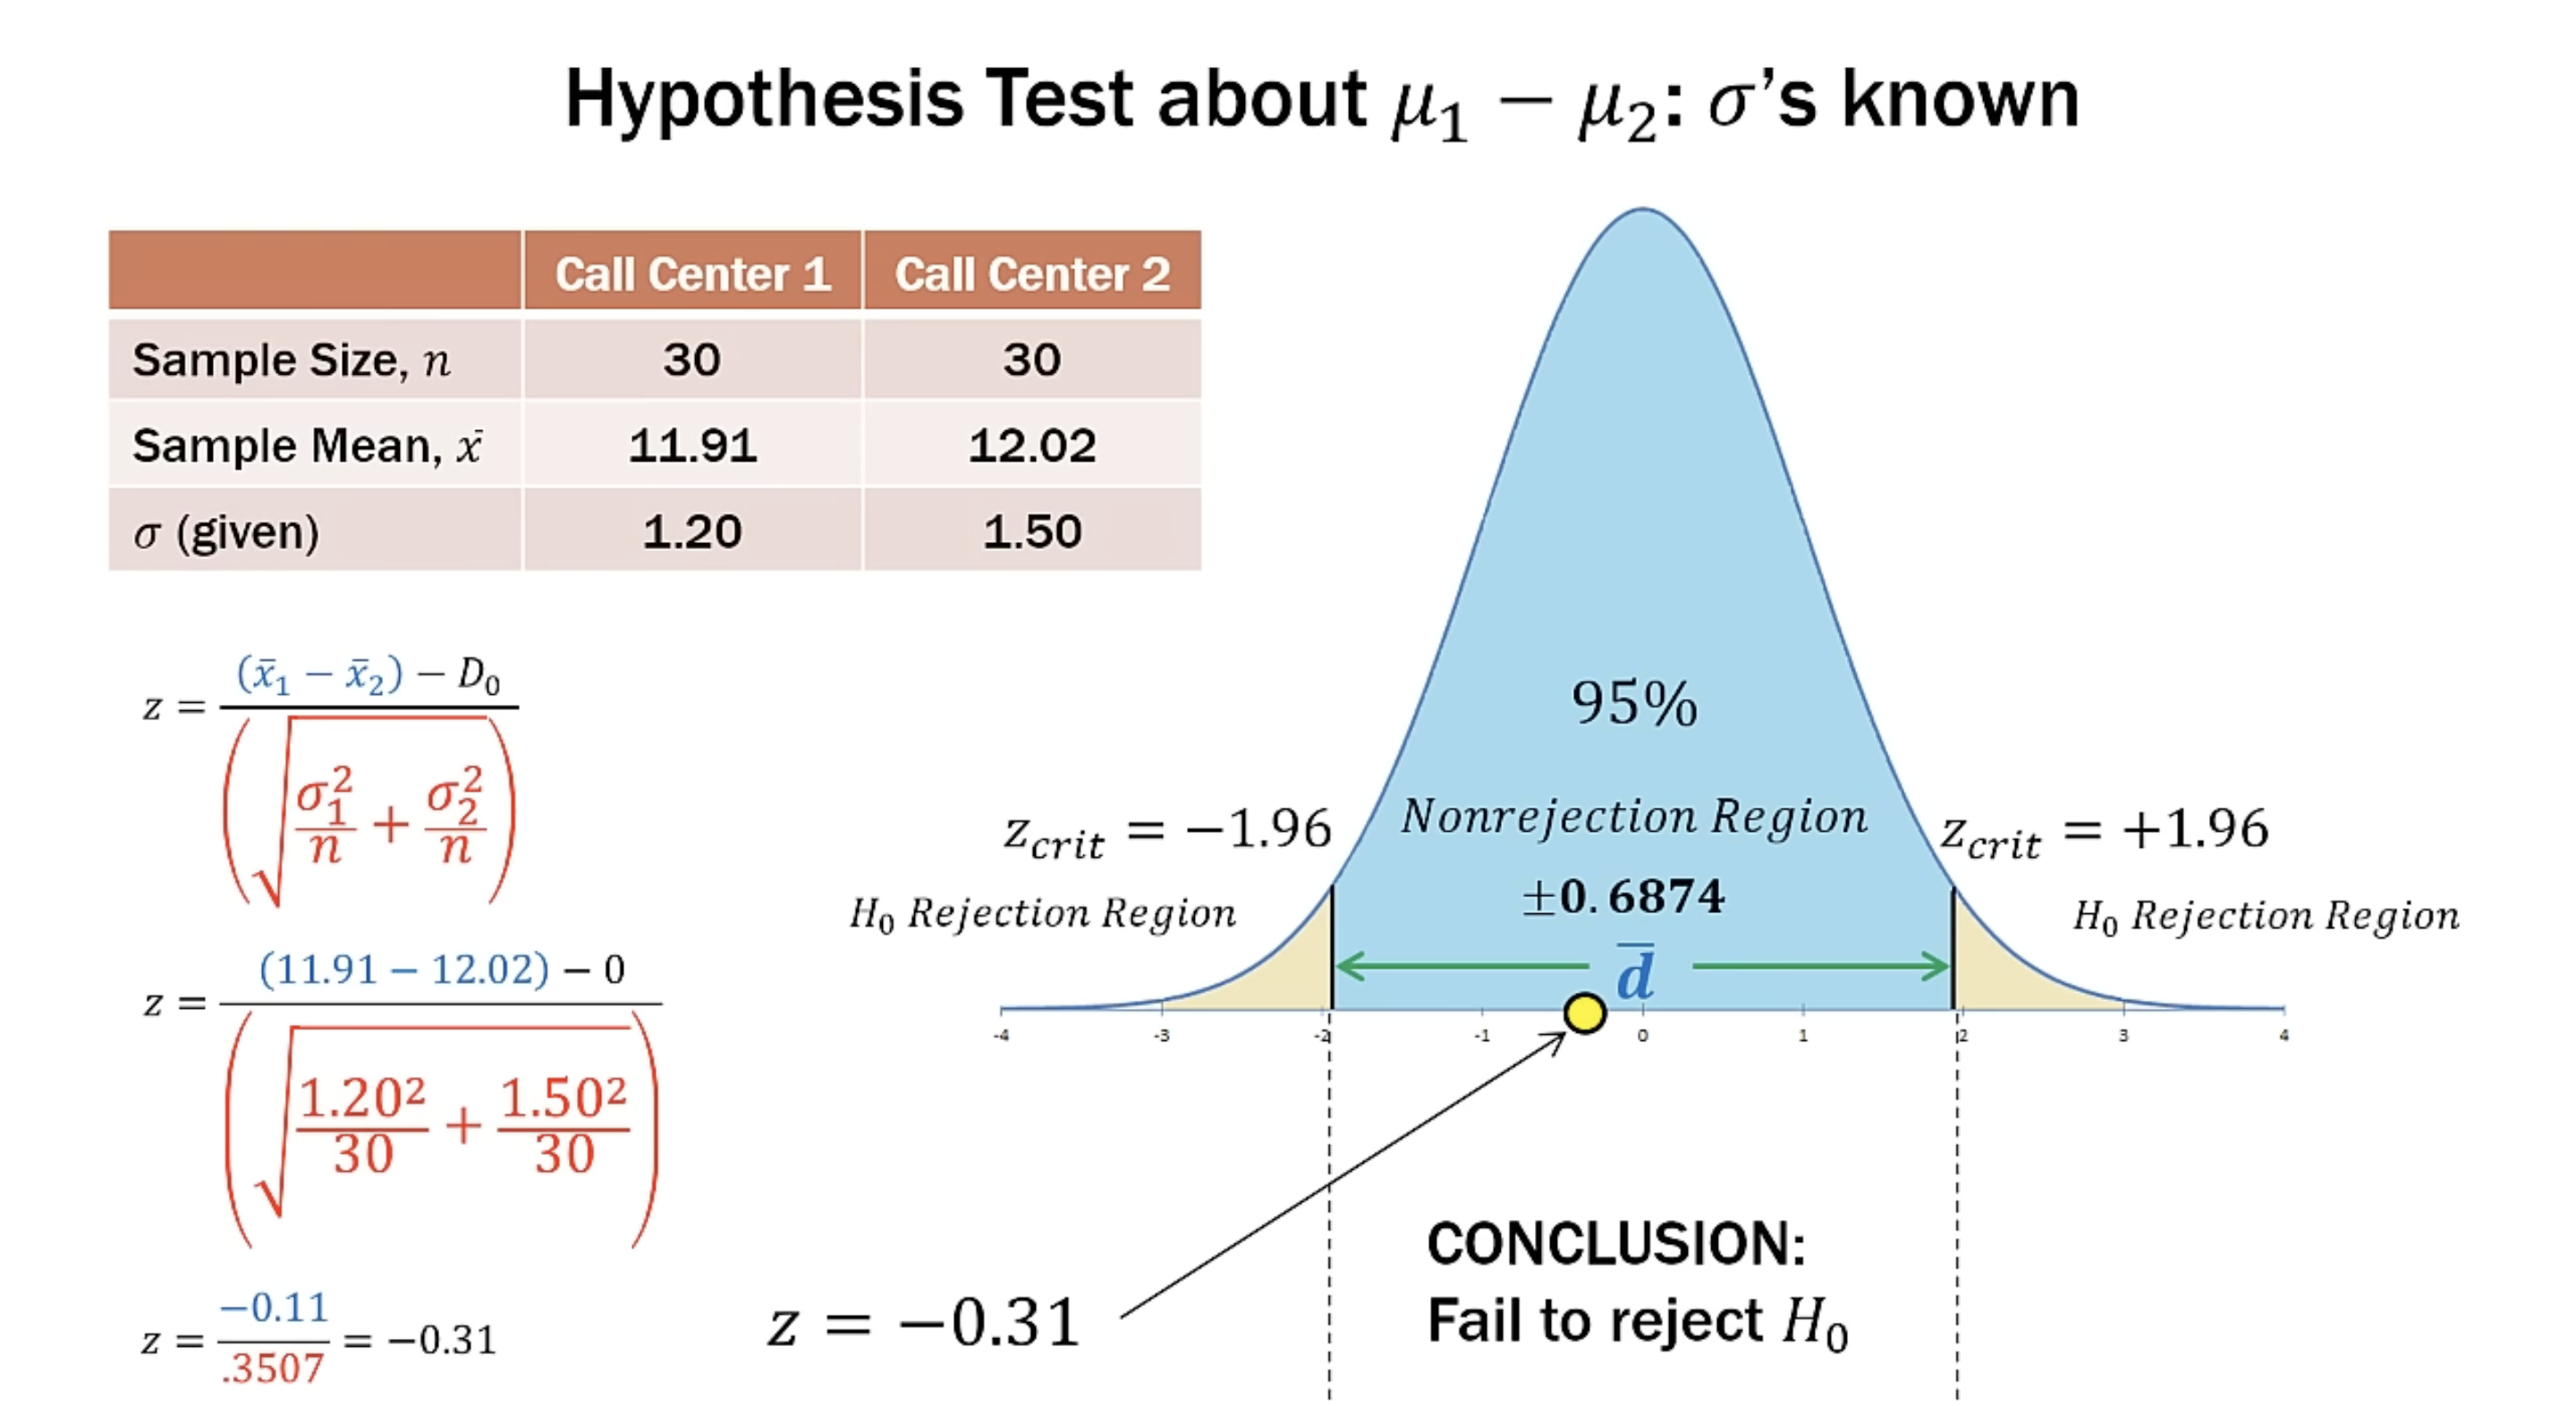
\includegraphics[width=1\linewidth]{2sampzexample.png}
\end{figure}

\begin{itemize}
    \item When we are looking to differentiate or compare two distributions, we can compare their means or their variances
    \item \textbf{Formats} (where $D_0$ is hypothesized difference):
    \begin{itemize}
        \item Two-tailed:
        \begin{itemize}
            \item $H_0: \mu_1 - \mu_2 = D_0$
            \item $H_a: \mu_1 - \mu_2 \ne D_0$
        \end{itemize}
        \item One-tailed upper:
        \begin{itemize}
            \item $H_0: \mu_1 - \mu_2 \leq D_0$
            \item $H_a: \mu_1 - \mu_2 > D_0$
        \end{itemize}
        \item One-tailed lower:
        \begin{itemize}
            \item $H_0: \mu_1 - \mu_2 \geq D_0$
            \item $H_a: \mu_1 - \mu_2 < D_0$
        \end{itemize}
    \end{itemize}
     \item Z-test for difference of two independent random samples
    \begin{itemize}
        \item $z=\frac{\bar{x_1} - \bar{x_2} - D_0}{\sqrt{\frac{\sigma_1^2}{n}+\frac{\sigma_2^2}{n}}}$
        \item $\bar{x_1}, \bar{x_2}$ sample means
        \item $D_0$ hypothesized difference between two population means
        \item $\sigma_1, \sigma_2$ population standard deviations
        \item $n$ sample size
    \end{itemize}
    \item Interval estimate of the difference for two independent random samples $=\bar{d} \pm \text{margin of error}$
    \item $=\bar{d} \pm z_{\alpha/2} \cdot (\sqrt{\frac{\sigma_1^2}{n}+\frac{\sigma_2^2}{n}})$
    \item Find $z_{\alpha/2}$ on \textbf{TI84}: \code{DISTR -> invNorm} \code{area:1-$\alpha/2$ tail:LEFT}
\end{itemize}

\subsection{Two Populations T-test}

\begin{figure}[H]
    \centering
    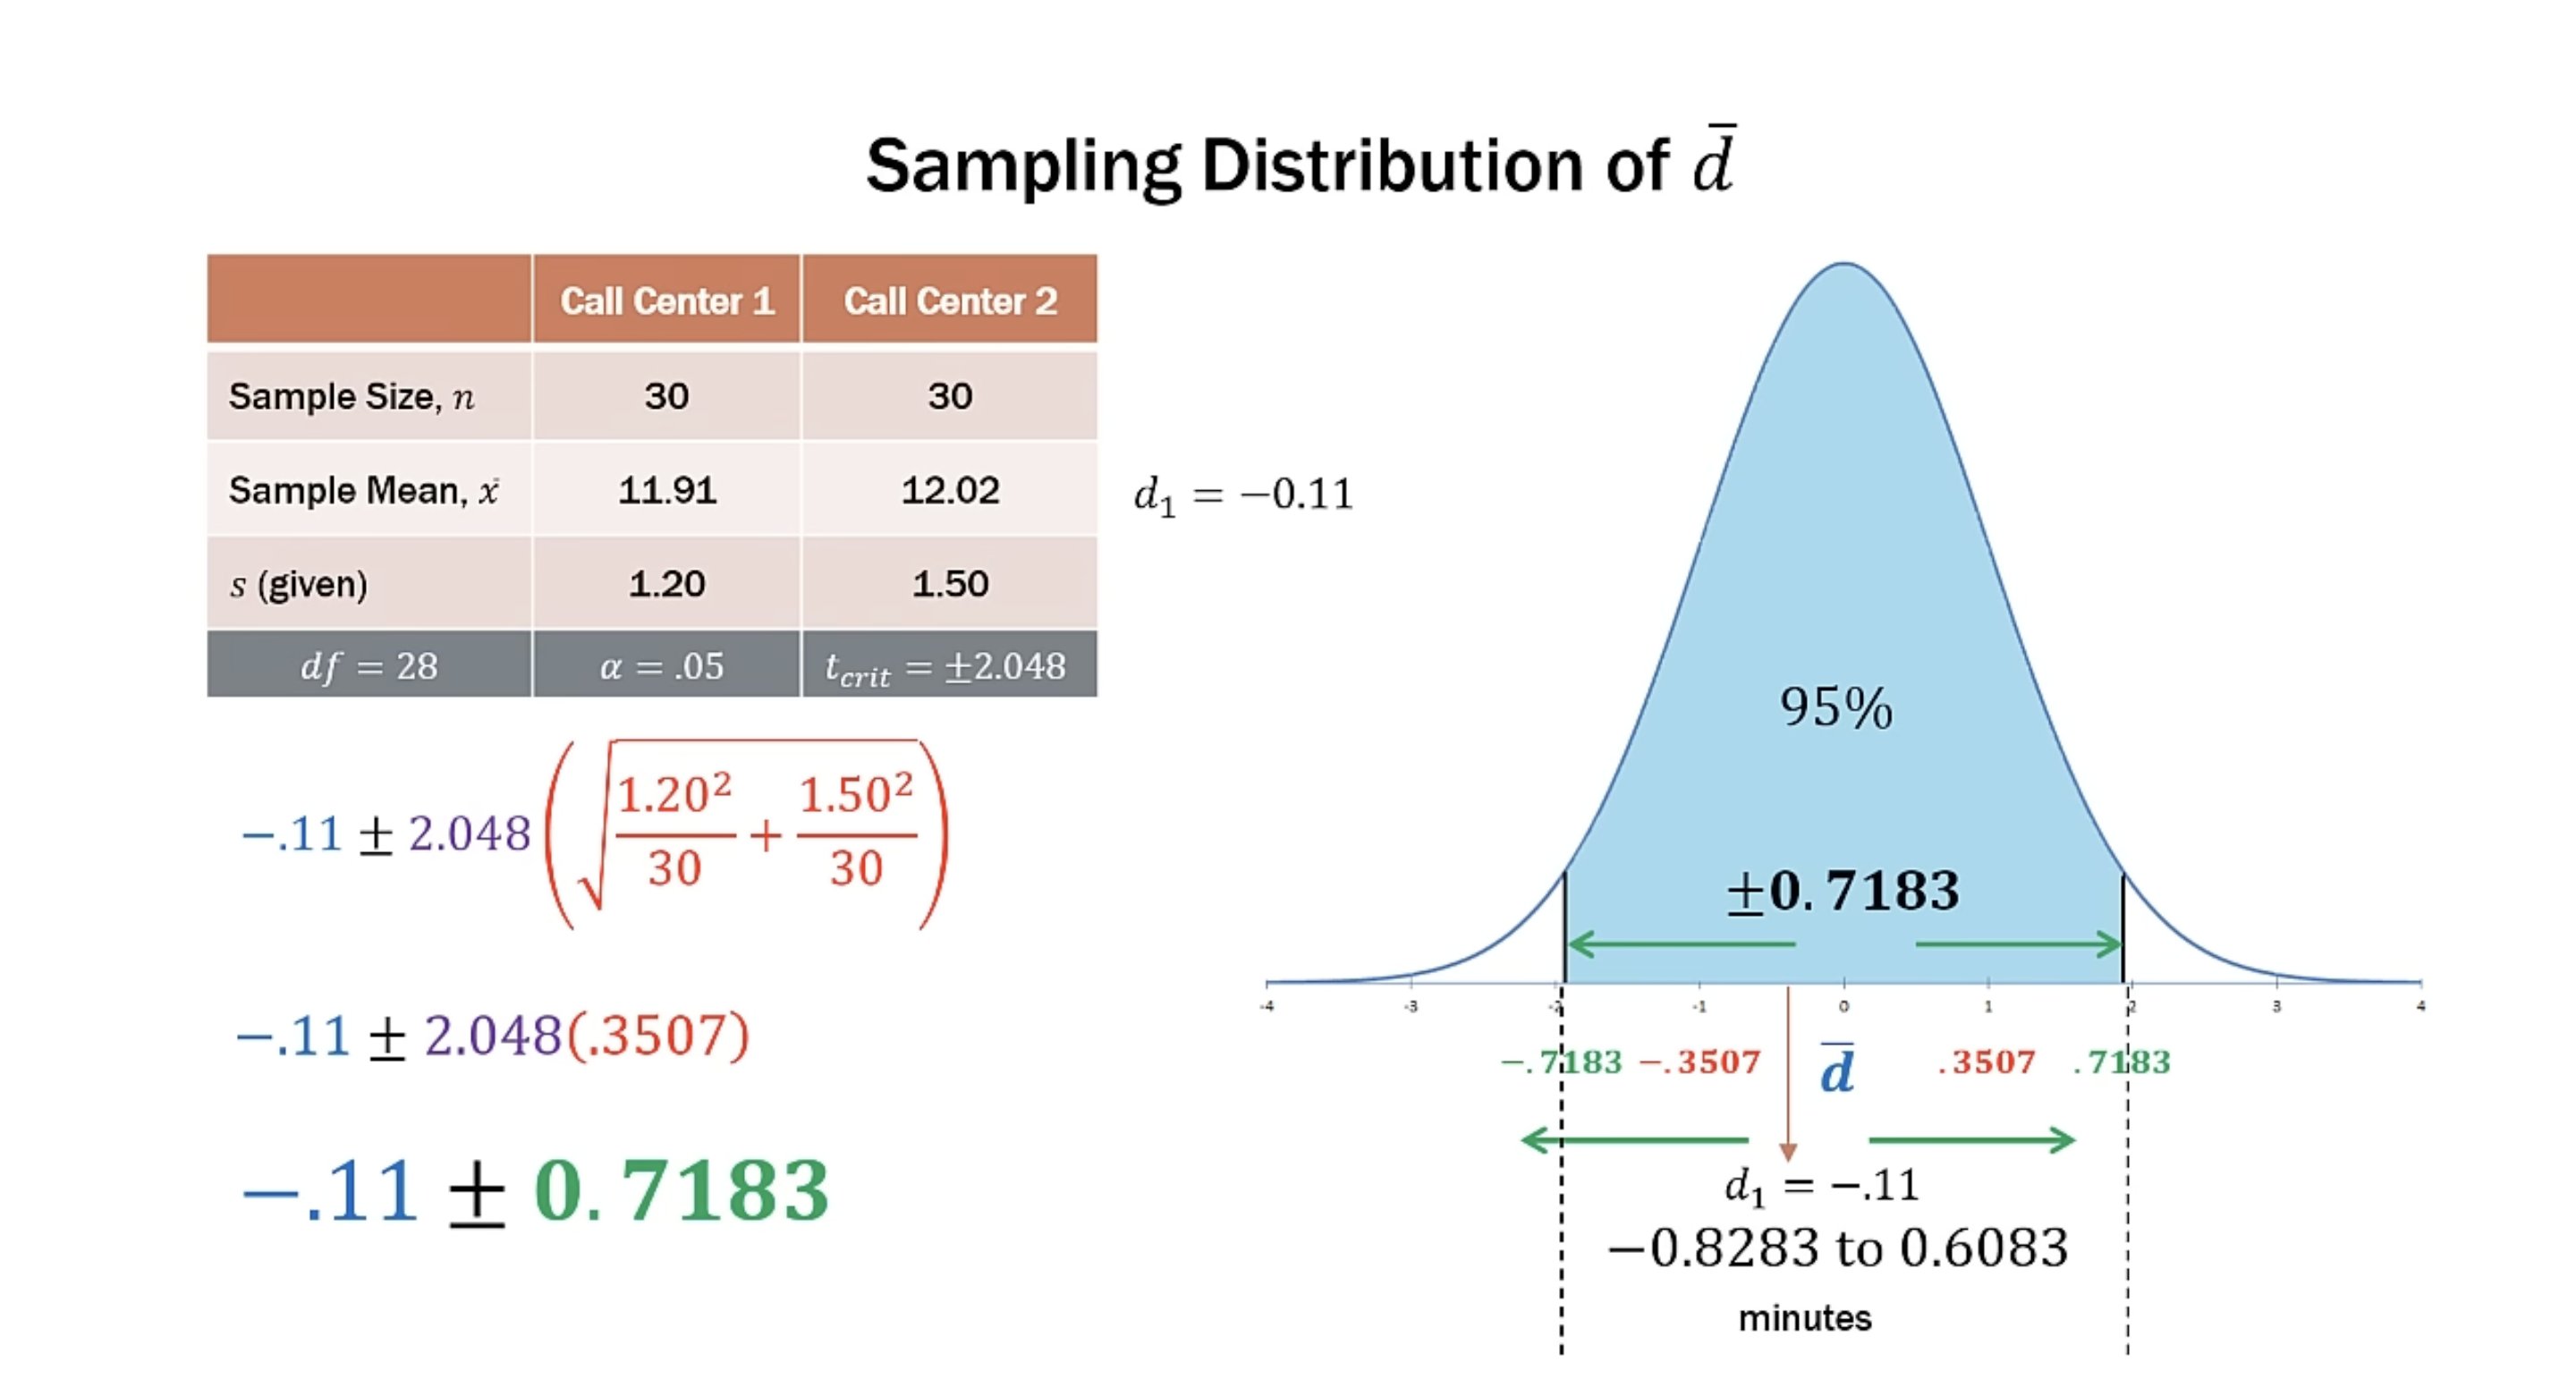
\includegraphics[width=1\linewidth]{2samptexample.png}
\end{figure}

\begin{itemize}
    \item Similar principles as Two Populations Z-test
    \item When the population standard deviations, $\sigma$, are unknown we must estimate using the sample standard deviation, $s$; thus, we switch to using the $t$-distribution with a certain degrees of freedom
    \item \textbf{Distribution of differences}:
    \begin{enumerate}
        \item Take an independent sample from $u_1$ which will be $\bar{x_1}$
        \item Take an independent sample from $u_2$ which will be $\bar{x_2}$
        \item Find $\bar{x_1}-\bar{x_2}=d_i$ (difference)
        \item Repeat process
        \item Create a distribution of the differences, $d_i$ 
    \end{enumerate}
    \item $\bar{x_1}-\bar{x_2}$ or $d$ is a point estimator of $\mu_1-\mu_2$
    \item After doing steps above, you can calculate mean of the differences $\bar{d}$
    \item Standard Error of the Difference for Two Independent Random Samples $s_{\bar{d}}=s_{\bar{x_1}-\bar{x_2}}=\sqrt{\frac{s_1^2}{n_1}+\frac{s_2^2}{n_2}}$
    \item Interval estimate of the difference for two independent random samples $=\bar{d} \pm \text{margin of error}$
    \item $=\bar{d} \pm t_{\alpha/2} \cdot (\sqrt{\frac{s^2}{n}+\frac{s^2}{n}})$
    \item $df=\frac{\frac{s_1^2}{n_1}+\frac{s_2^2}{n_2}}{\frac{1}{n_1-1}\frac{s_1^2}{n_1}+\frac{1}{n_2-1}\frac{s_2^2}{n_2}}$
    \item Find $t_{\alpha/2}$ on \textbf{TI84}: \code{DISTR -> invT} \code{area:1-$\alpha/2$}
\end{itemize}

\subsection{Two Populations Matched Sample T-test}

\begin{figure}[H]
        \centering
        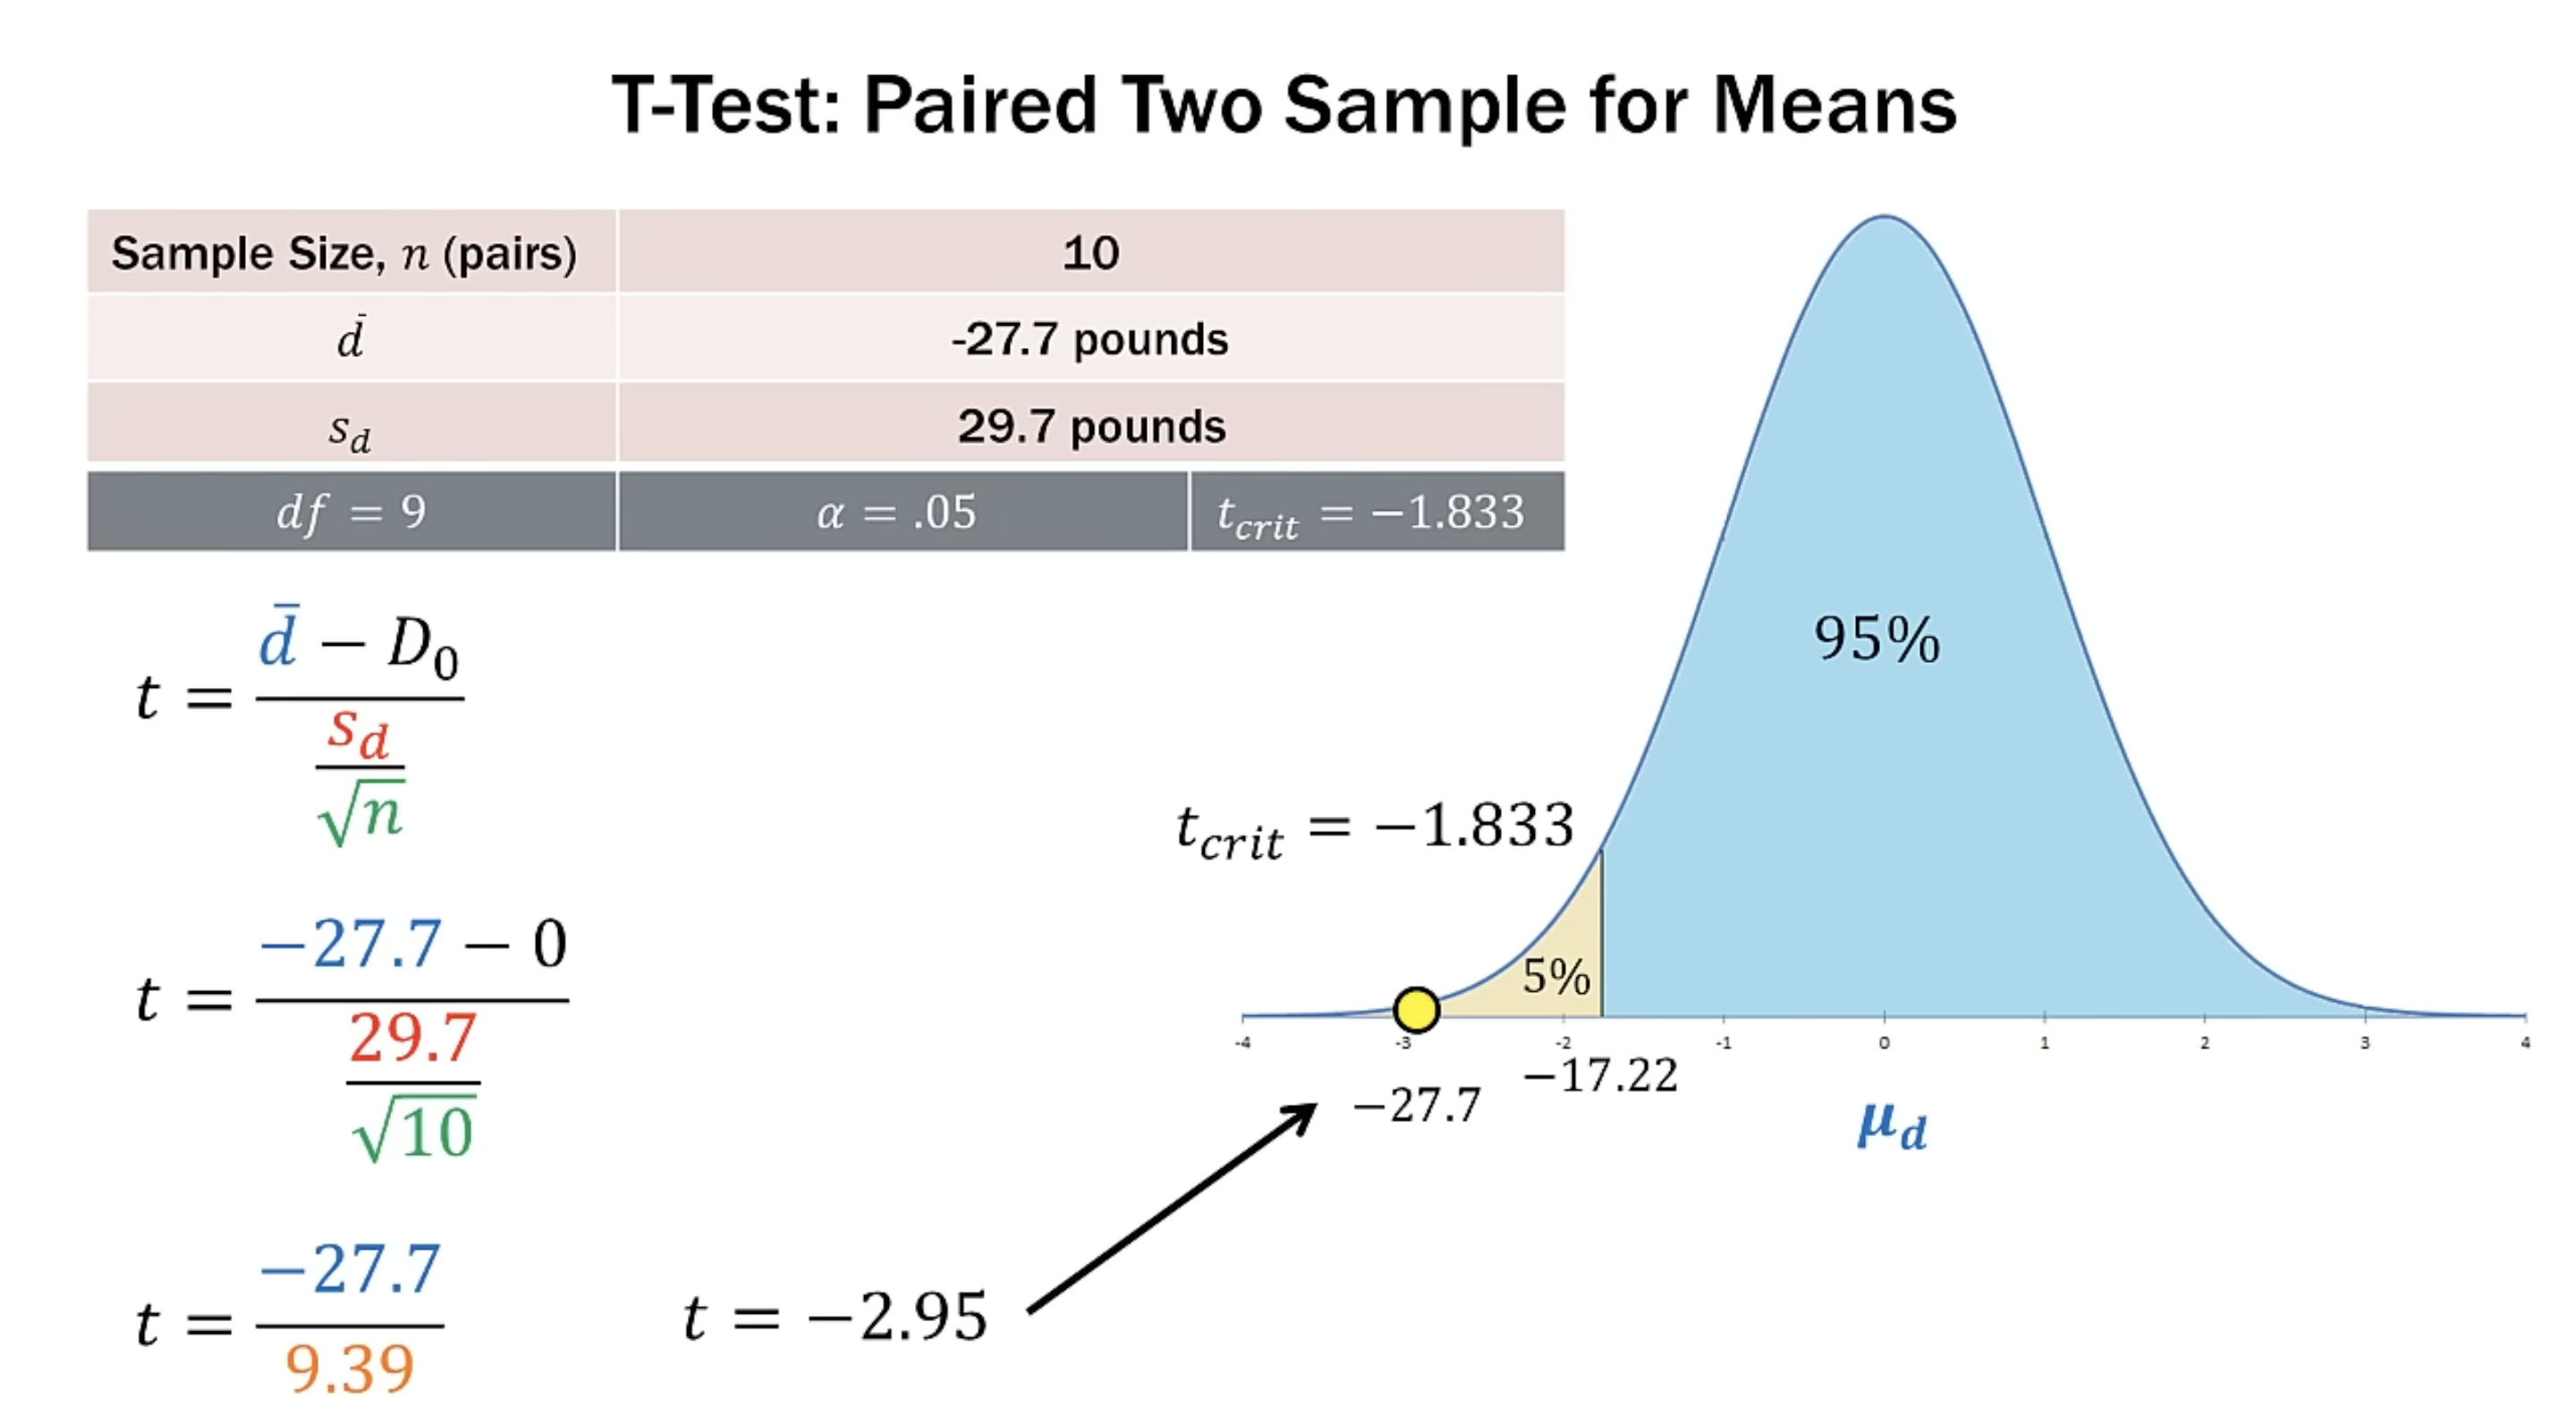
\includegraphics[width=1\linewidth]{matchedtexample.png}
    \end{figure}

\begin{itemize}
    \item Method for when samples are not independent
    \item For example, doing a performance test before and after a training session
    \item $d_i$ (differences between $x_1i$ and $x_2i$) form sampling distribution, with $\bar{d}=\text{mean of the differences}$ and $s_d=\text{std dev of differences}$ 
    \item Standard Error of the difference for two matched measurements $s_{\bar{d}}=\frac{s_d}{\sqrt{n}}$ where $s_d$ is the standard deviation of the differences
    \item Matched Pair $t$-Test $t=\frac{\bar{d}-\mu_d}{s_d/\sqrt{n}}, df=n-1$ where $\mu_d$ is the hypothesized mean difference
    \item Interval estimate of the difference for two matched measurements $=\bar{d} \pm \text{margin of error}$
    \item $=\bar{d} \pm t_{\alpha/2} \frac{s_d}{\sqrt{n}}$ (two tailed)
\end{itemize}

\section{Goodness of Fit and Independence Tests}

\subsection{Chi-square test}

\begin{itemize}
    \item A $\chi ^2$ test helps us understand the relationship between two categorical variables; i.e.: sex, age group, year, etc.
    \item Chi-squares involves the frequency of events; the count
    \item It helps us compare what we actually observed with what we expected often using population data or theoretical data
    \item Chi-squares help us determine the role of random chance variation between our categorical variables
    \item We use the Chi-square distribution and critical values to accept or reject our hypothesis
    \item $H_0: $ the variation in our data is simply observed due to chance
    \item $H_1: $ the variation is beyond what random chance should allow
    \item $\text{degrees of freedom} = n-1$
    \item \textbf{TI84}:
    \begin{enumerate}
        \item Fill in \code{L1} with observed and \code{L2} with expected
        \item Use \code{STAT -> TESTS -> $\chi^2$GOF-Test}
    \end{enumerate}
    \item \textbf{Manual}:
    \begin{enumerate}
        \item For each observation, calculate 
        $\frac{(\text{observed} - \text{expected})^2}{\text{expected}}$
        \item Sum all the values from 1. to get the $\chi^2$ value
        \item If our $\chi^2>\text{critical value}$, which we can find on page 493 of the textbook, we must reject $H_0$
    \end{enumerate}
    \item To estimate expected values when they're unknown: $\text{expected value} = \frac{\text{row total} \cdot \text{column total}}{n}$ (assuming typical cross-tabulation)
\end{itemize}

\section{Inferences about Population Variances}

\subsection{Variance and its Sampling Distribution}

\begin{itemize}
    \item Two or more data sets could have the same mean, but very different variances
    \item Population Variance: $\sigma^2 = \frac{\sum_{i=0}^{n}{(x_i-\mu)^2}}{N}$
    \item Sample Variance: $s^2 = \frac{\sum_{i=0}^{n}{(x_i-\bar{x})^2}}{n-1}$
    \item \textbf{Sampling Distribution of $s^2$}: When we take many samples of the same size from a normal population and then find those sample variances, $s^2$, those sample variances DO NOT follow the normal curve when placed in their own distribution, unlike sample means
    \item They follow the $\chi^2$ distribution, with $n-1$ degrees of freedom
    \item In the $\chi^2$ distribution, the cumulative probability runs right to left, not left to right, so at 0 it's 1
\end{itemize}

\subsection{Confidence Intervals for the Variance}

\begin{itemize}
    \item Whenever a random sample of size $n$ is selected from a normal population, the sampling distribution of:
    \begin{itemize}
        \item $\chi^2=\frac{(n-1)s^2}{\sigma^2}$
        \item $n=\text{sample size}$
        \item $s^2=\text{sample variance}$
        \item $\sigma^2=\text{population variance (unknown)}$
    \end{itemize}
    \item Increasing the sample size will narrow the interval estimate for the variance and standard deviation
    \item Interval estimates for variance are very sensitive to the overall population being normally distributed; check data first
    \item It's the variance that follows the chi-square distribution, not the standard deviation
\end{itemize}

\begin{figure}[H]
    \centering
    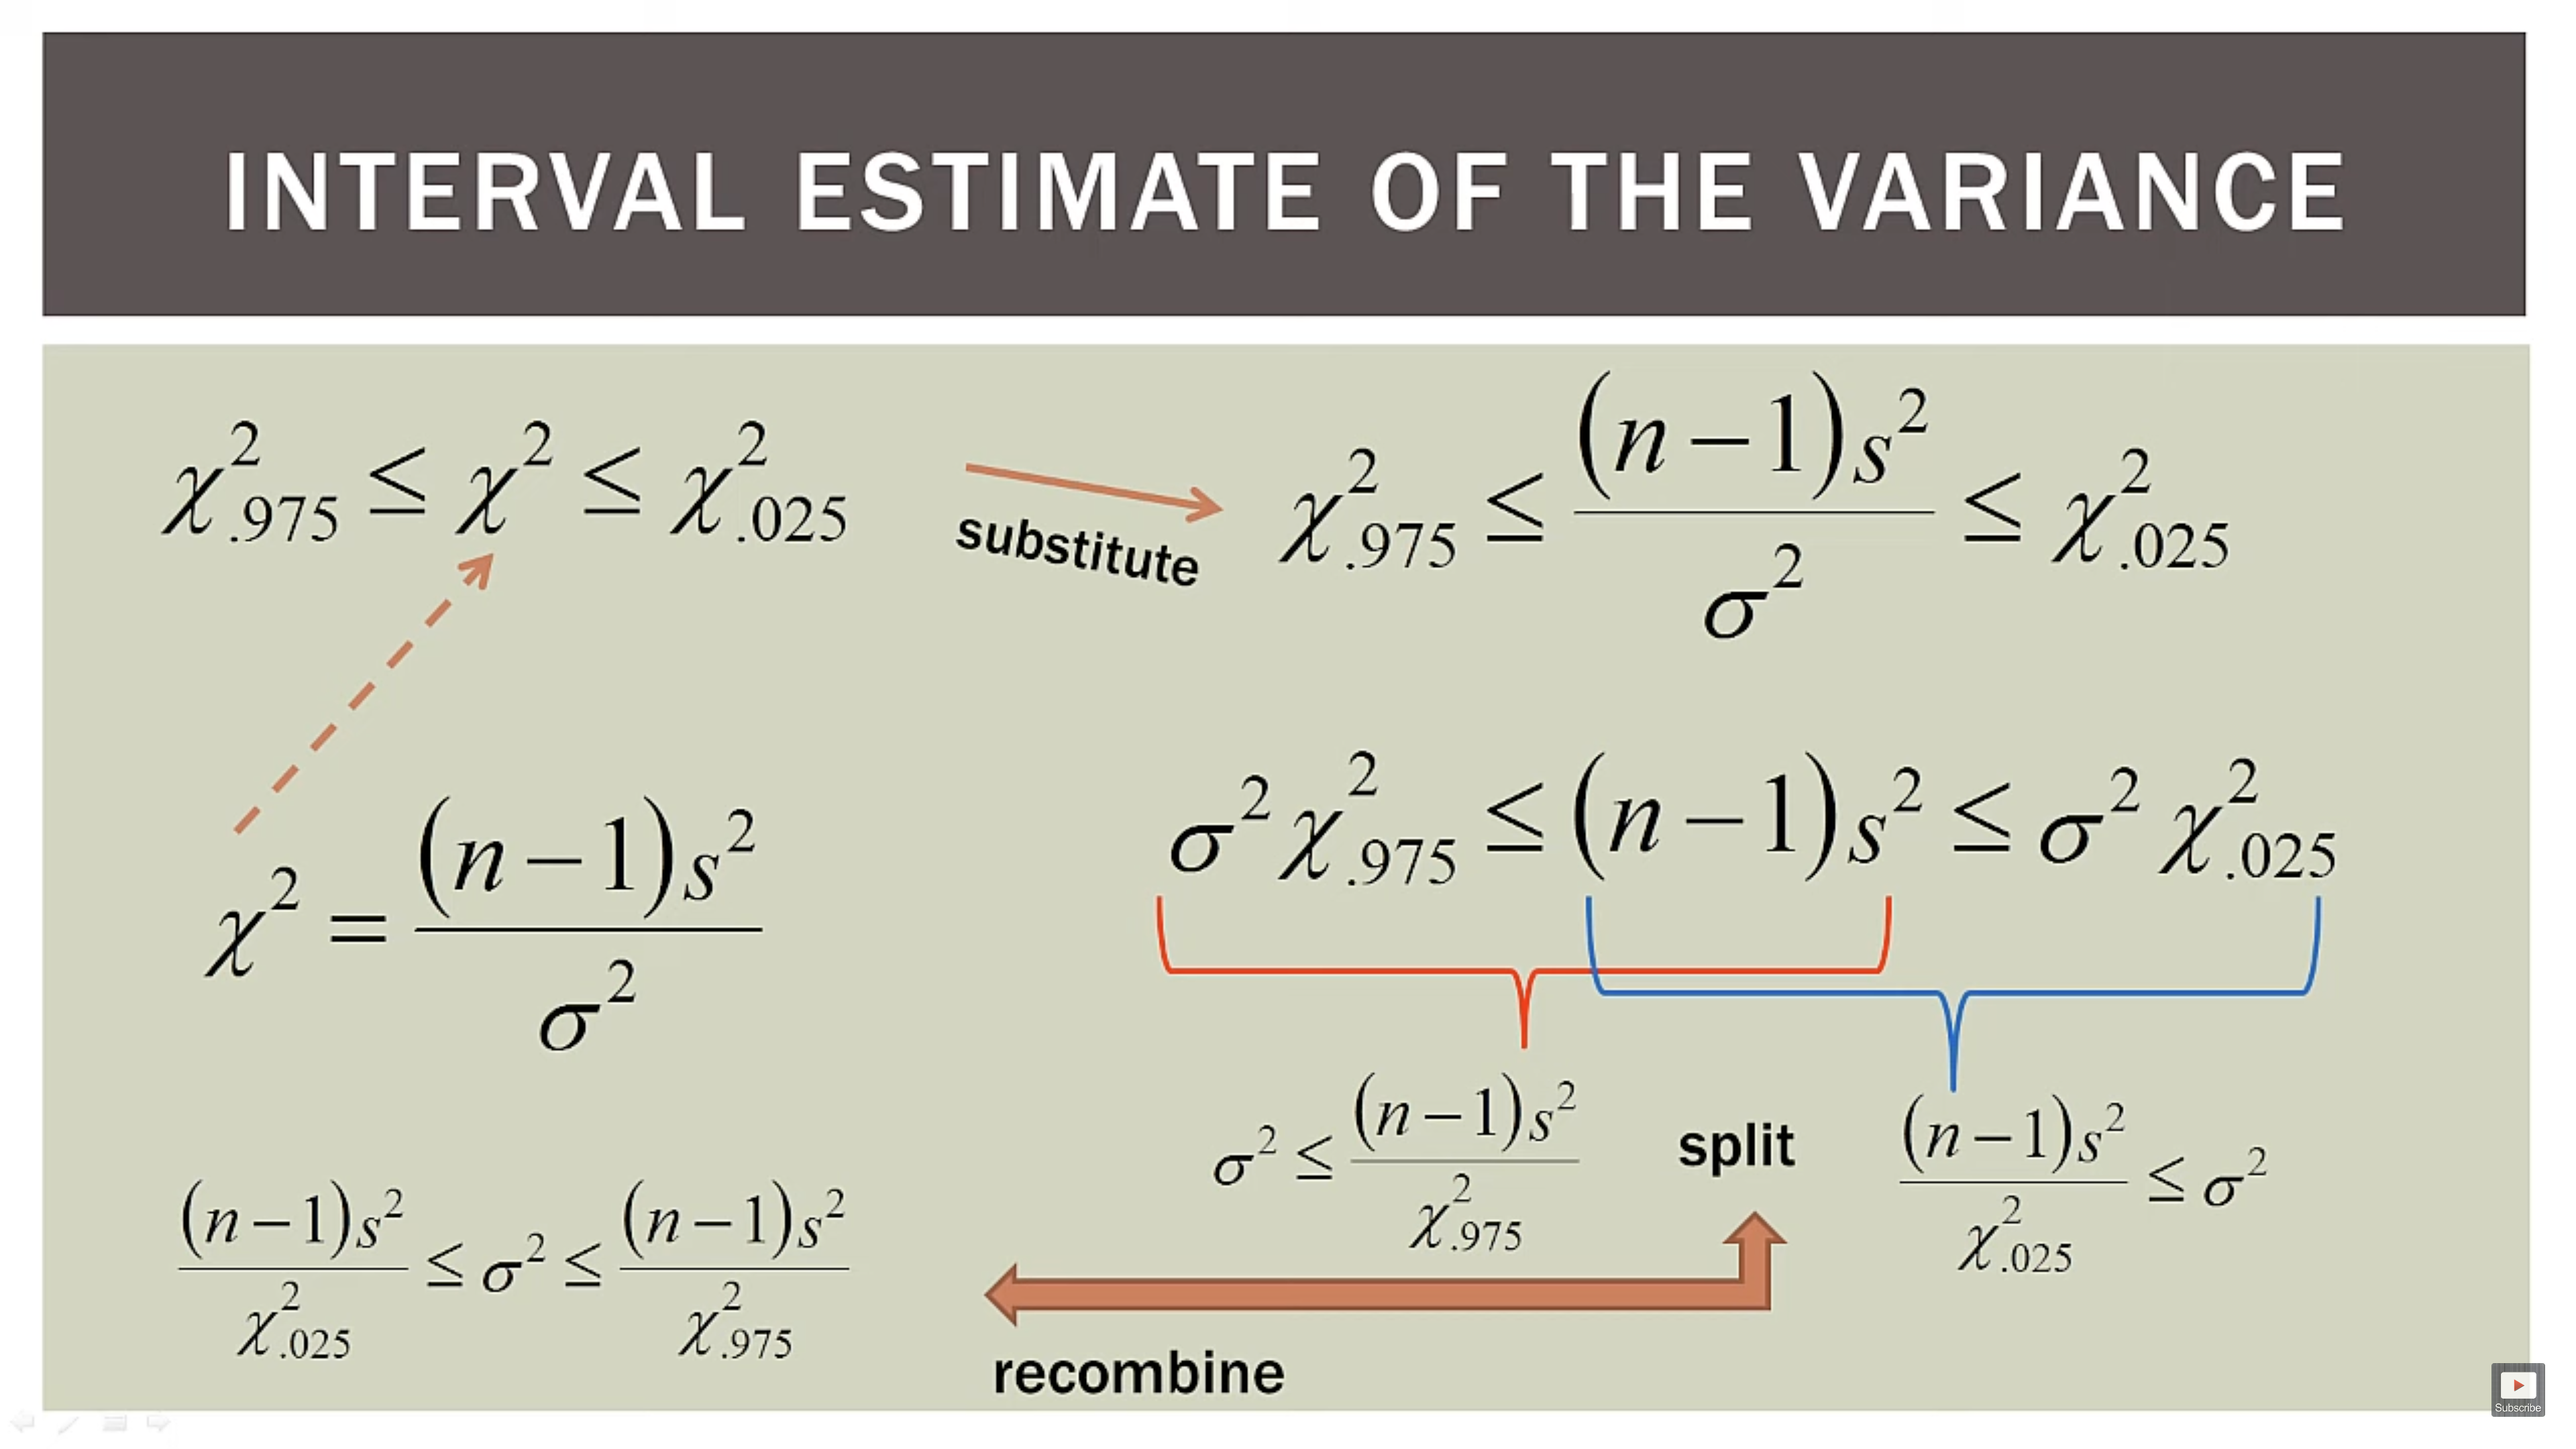
\includegraphics[width=0.45\linewidth]{civarianceexample.png}
    \hfill % This command adds space between the two figures
    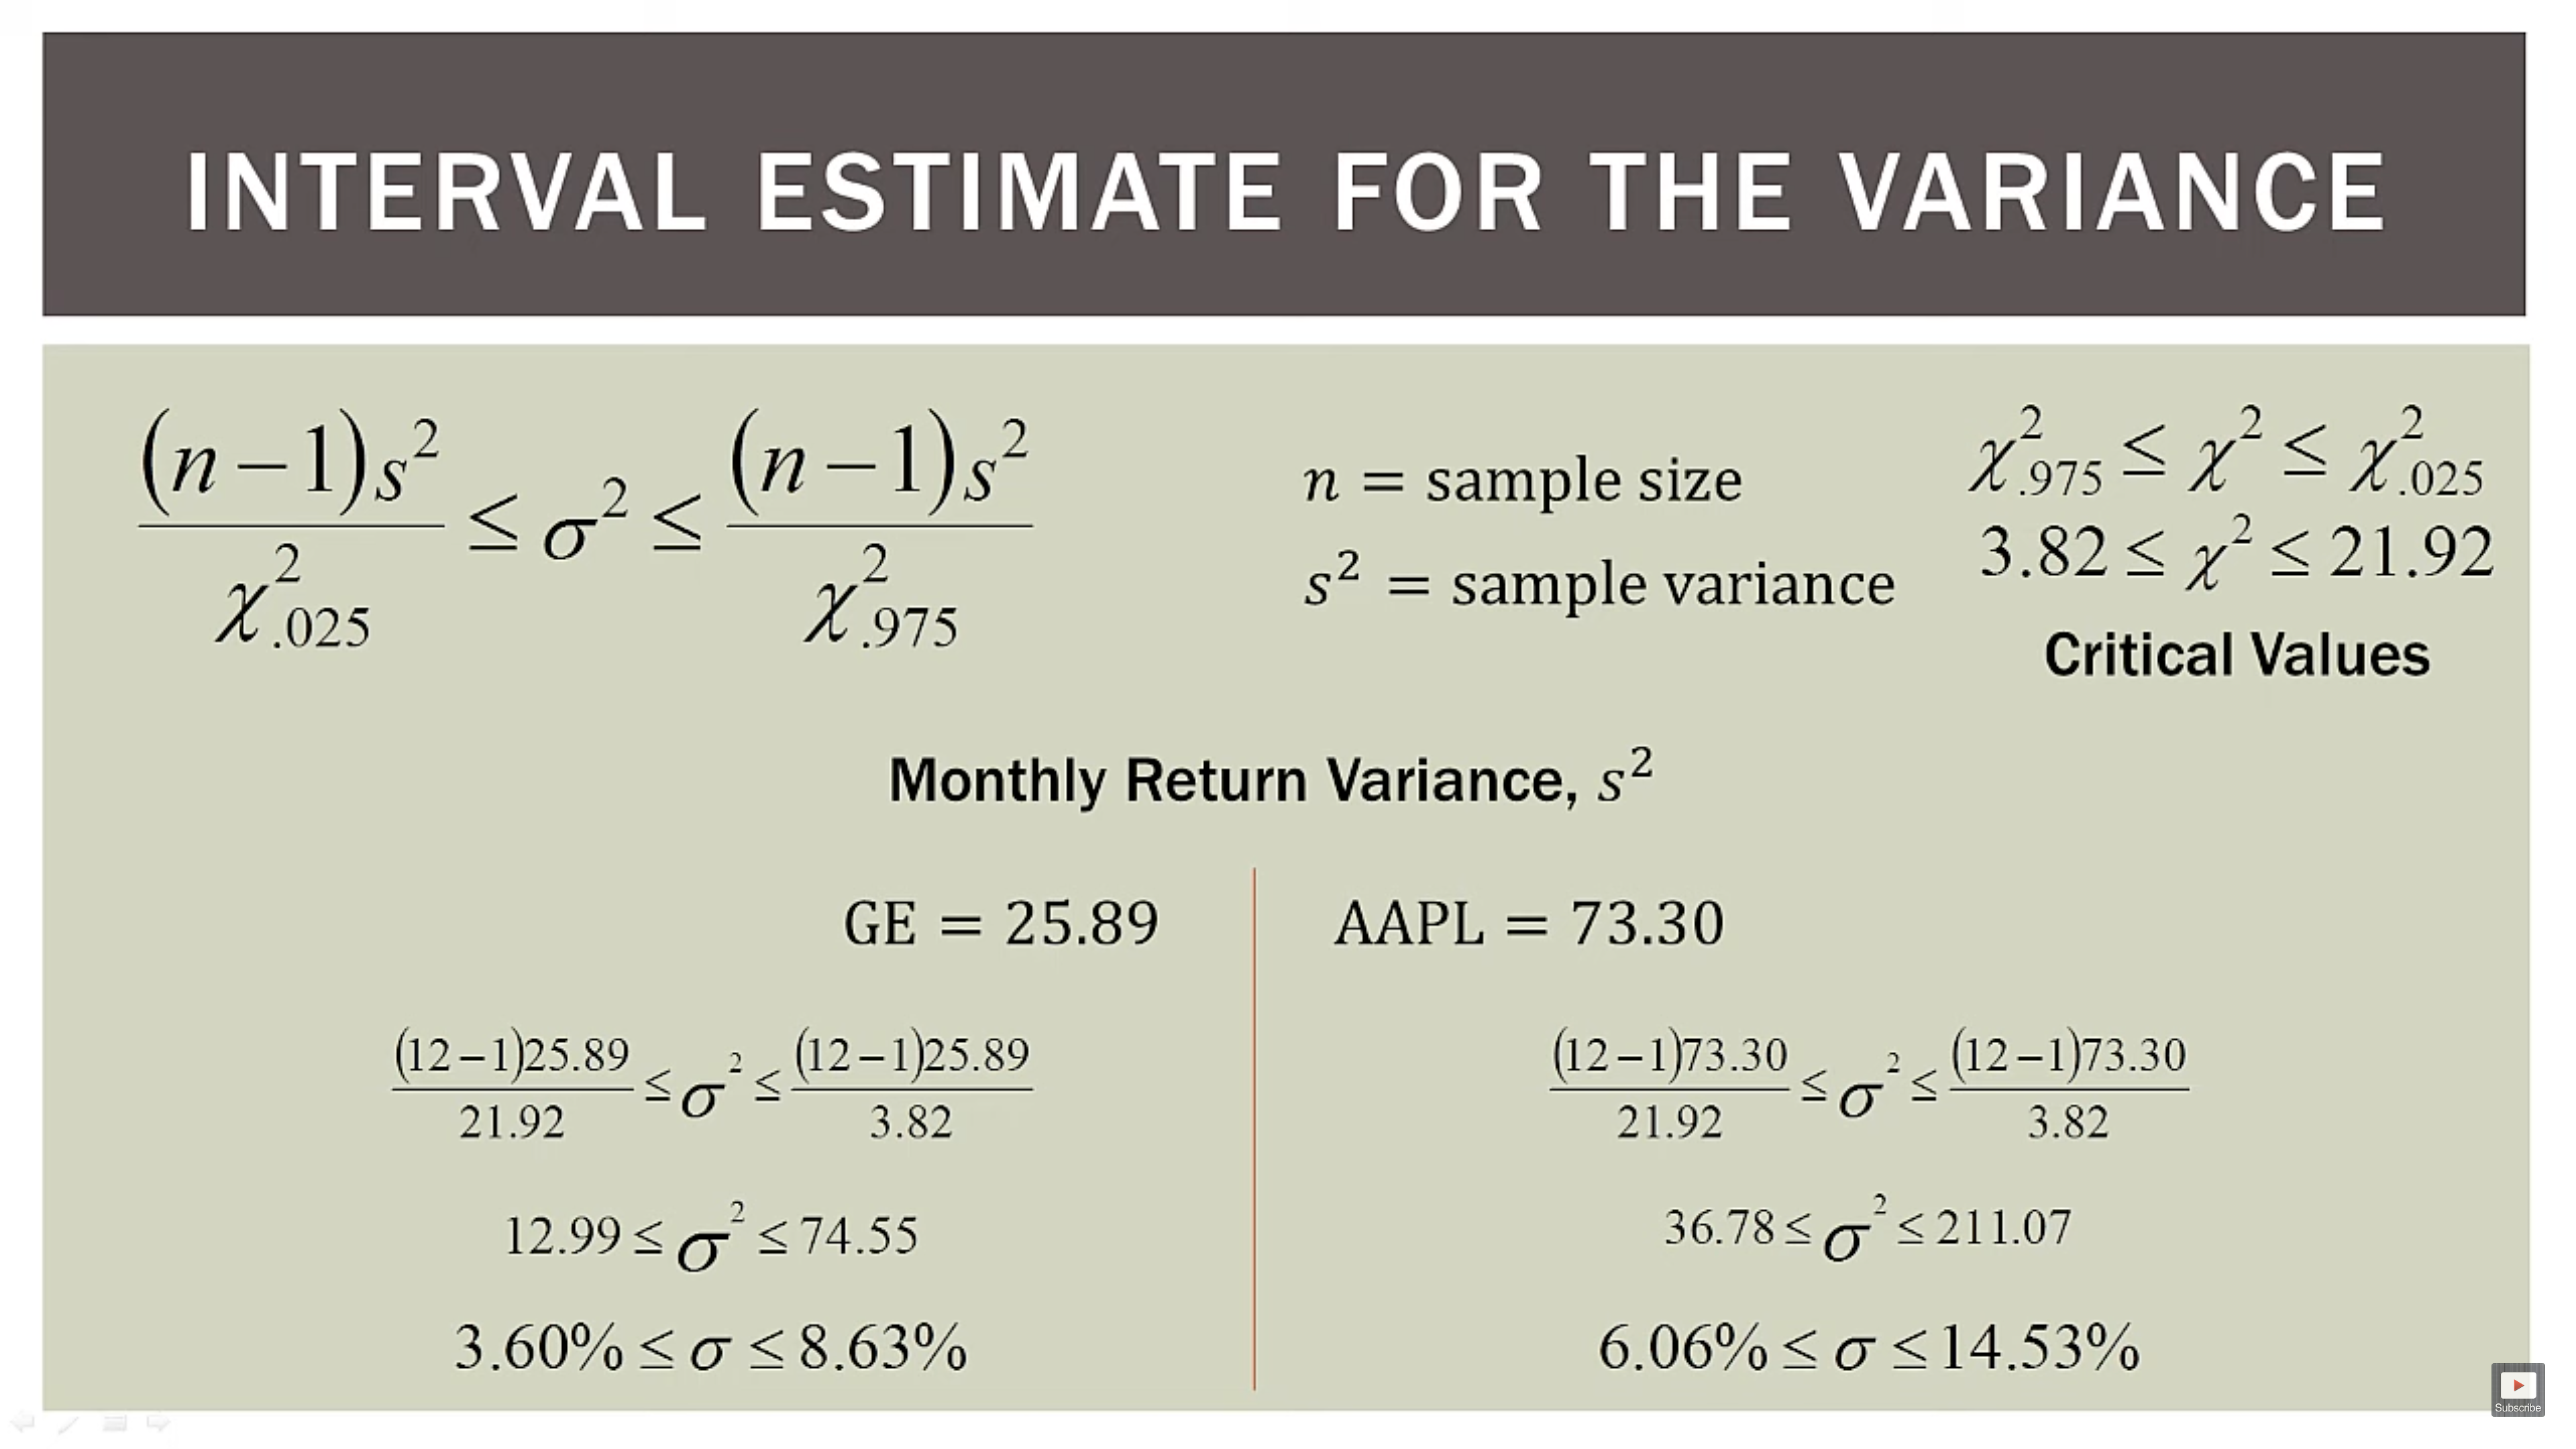
\includegraphics[width=0.45\linewidth]{civarianceexample2.png}
\end{figure}

\subsection{Hypothesis Tests for Variance}

\begin{figure}[H]
    \centering
    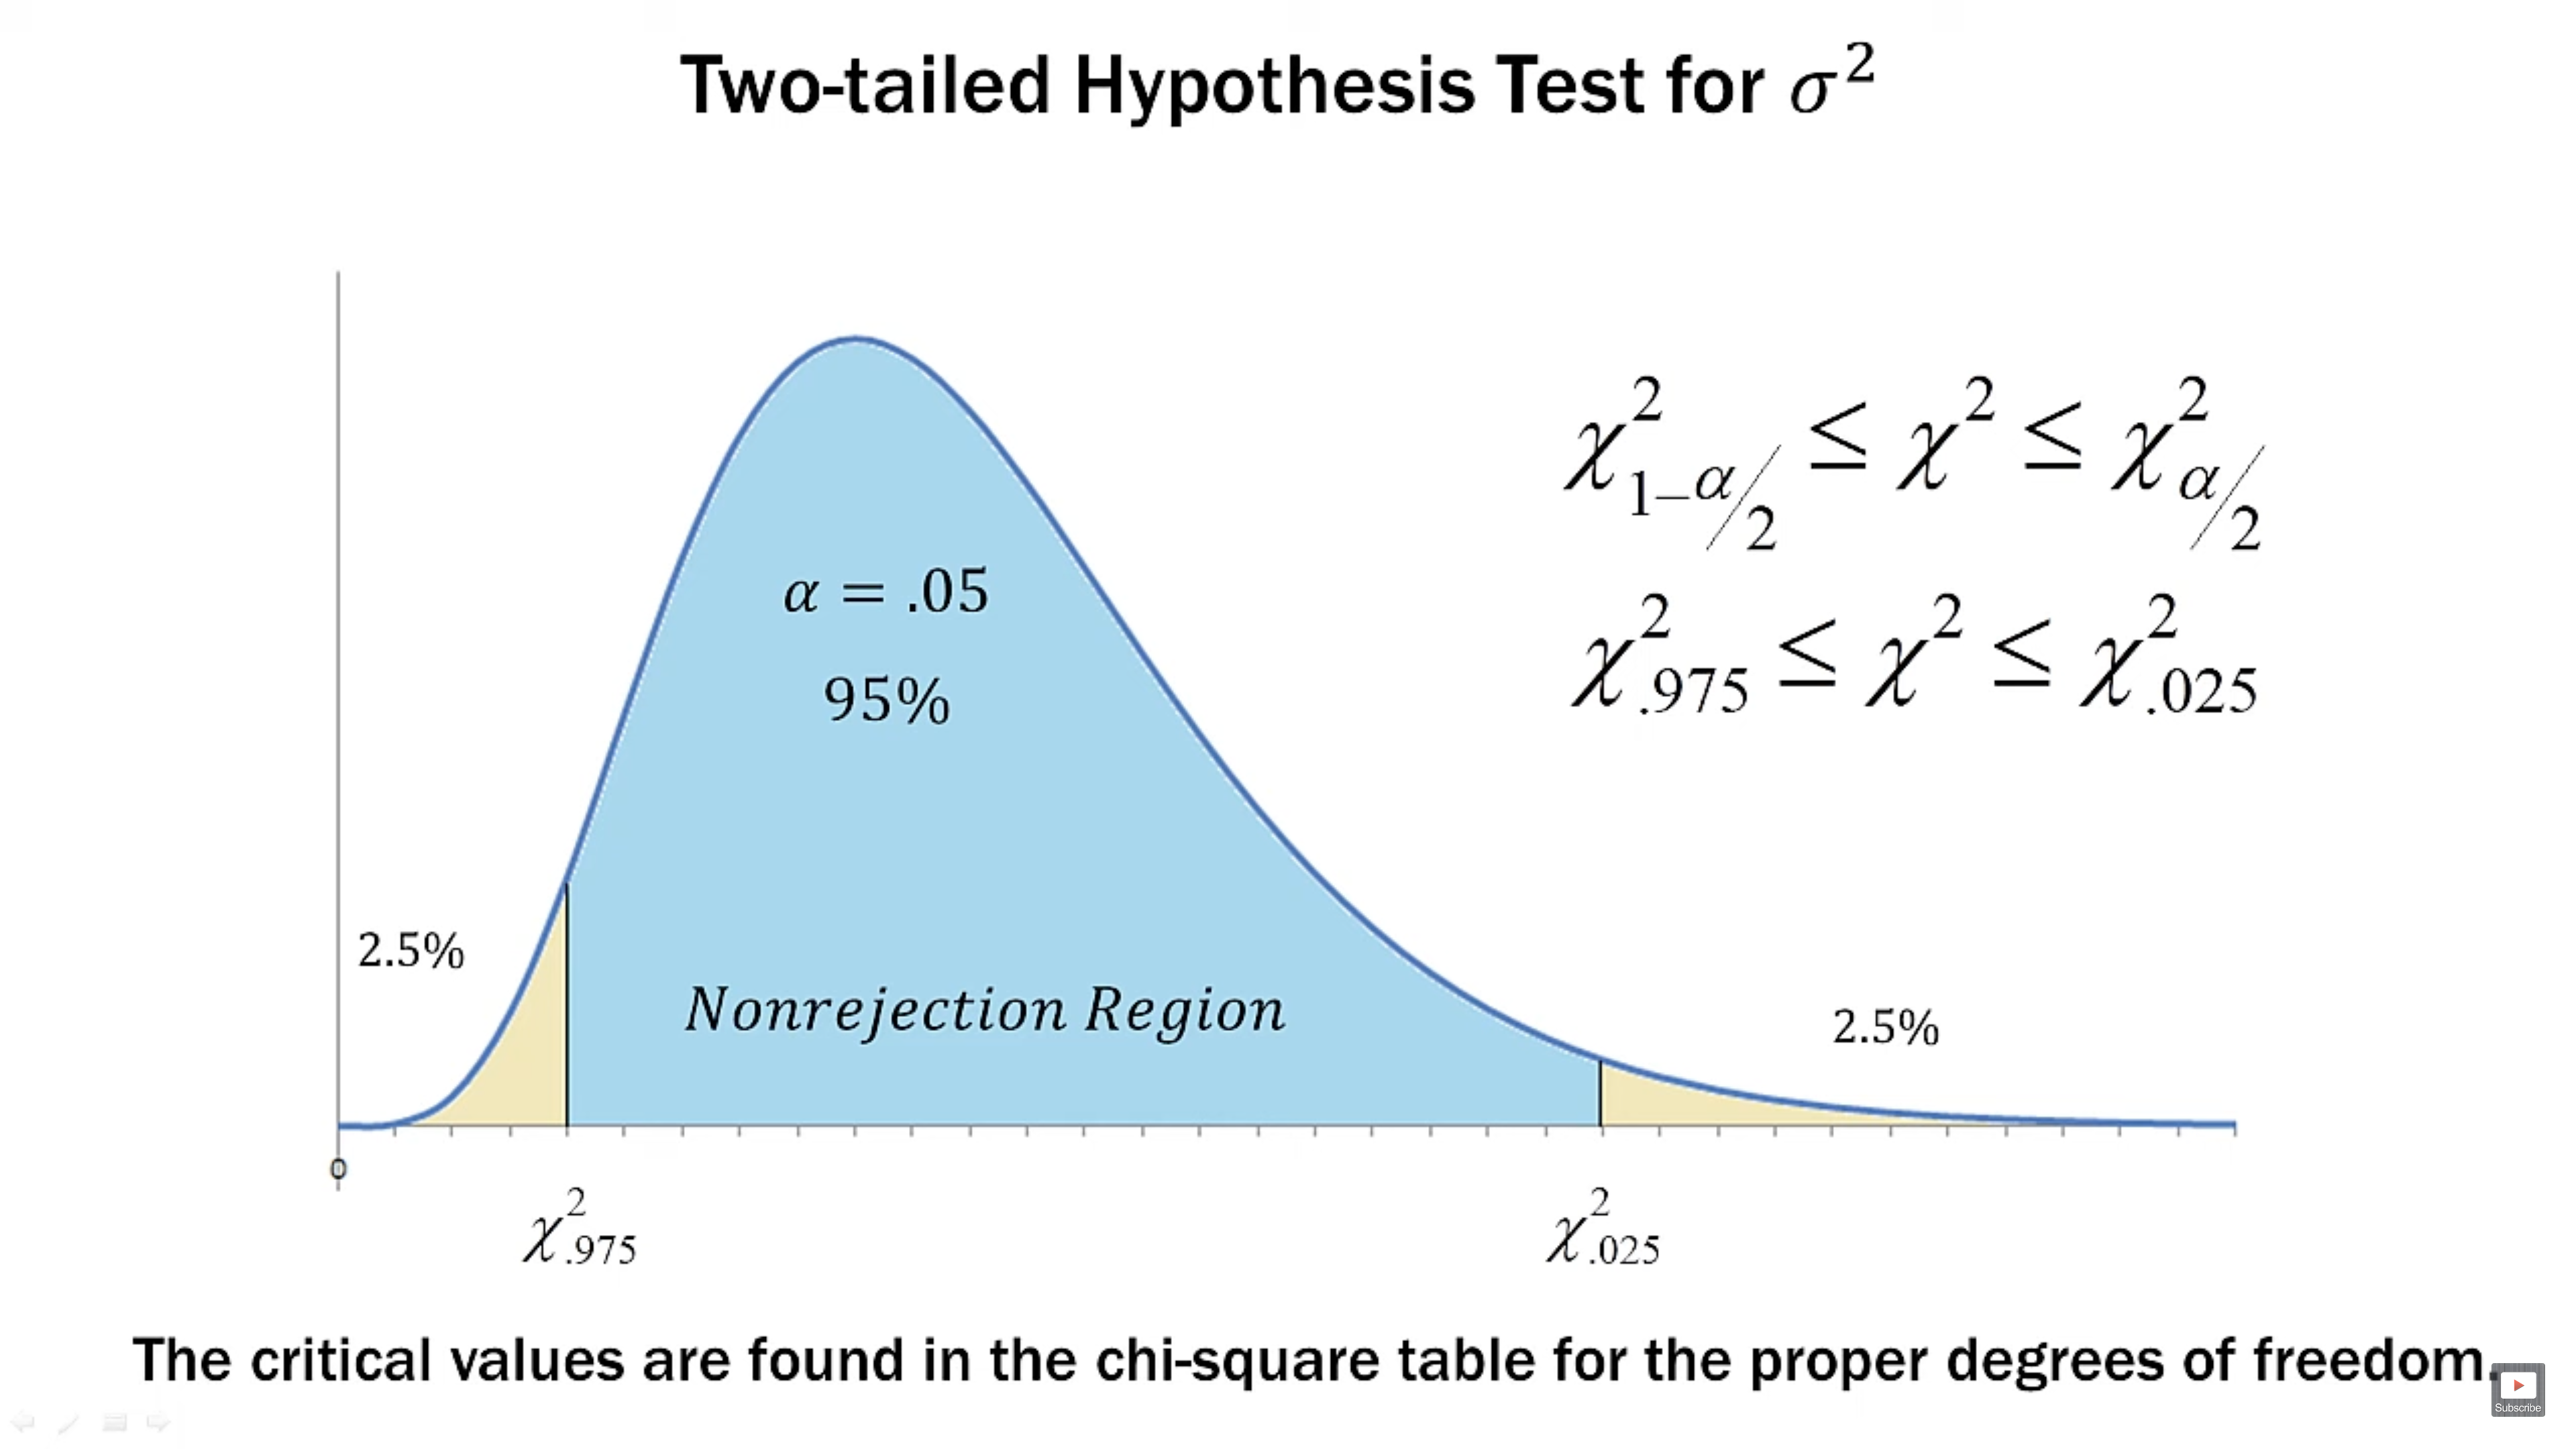
\includegraphics[width=0.45\linewidth]{varhtesttwotail.png}
    \hfill % This command adds space between the two figures
    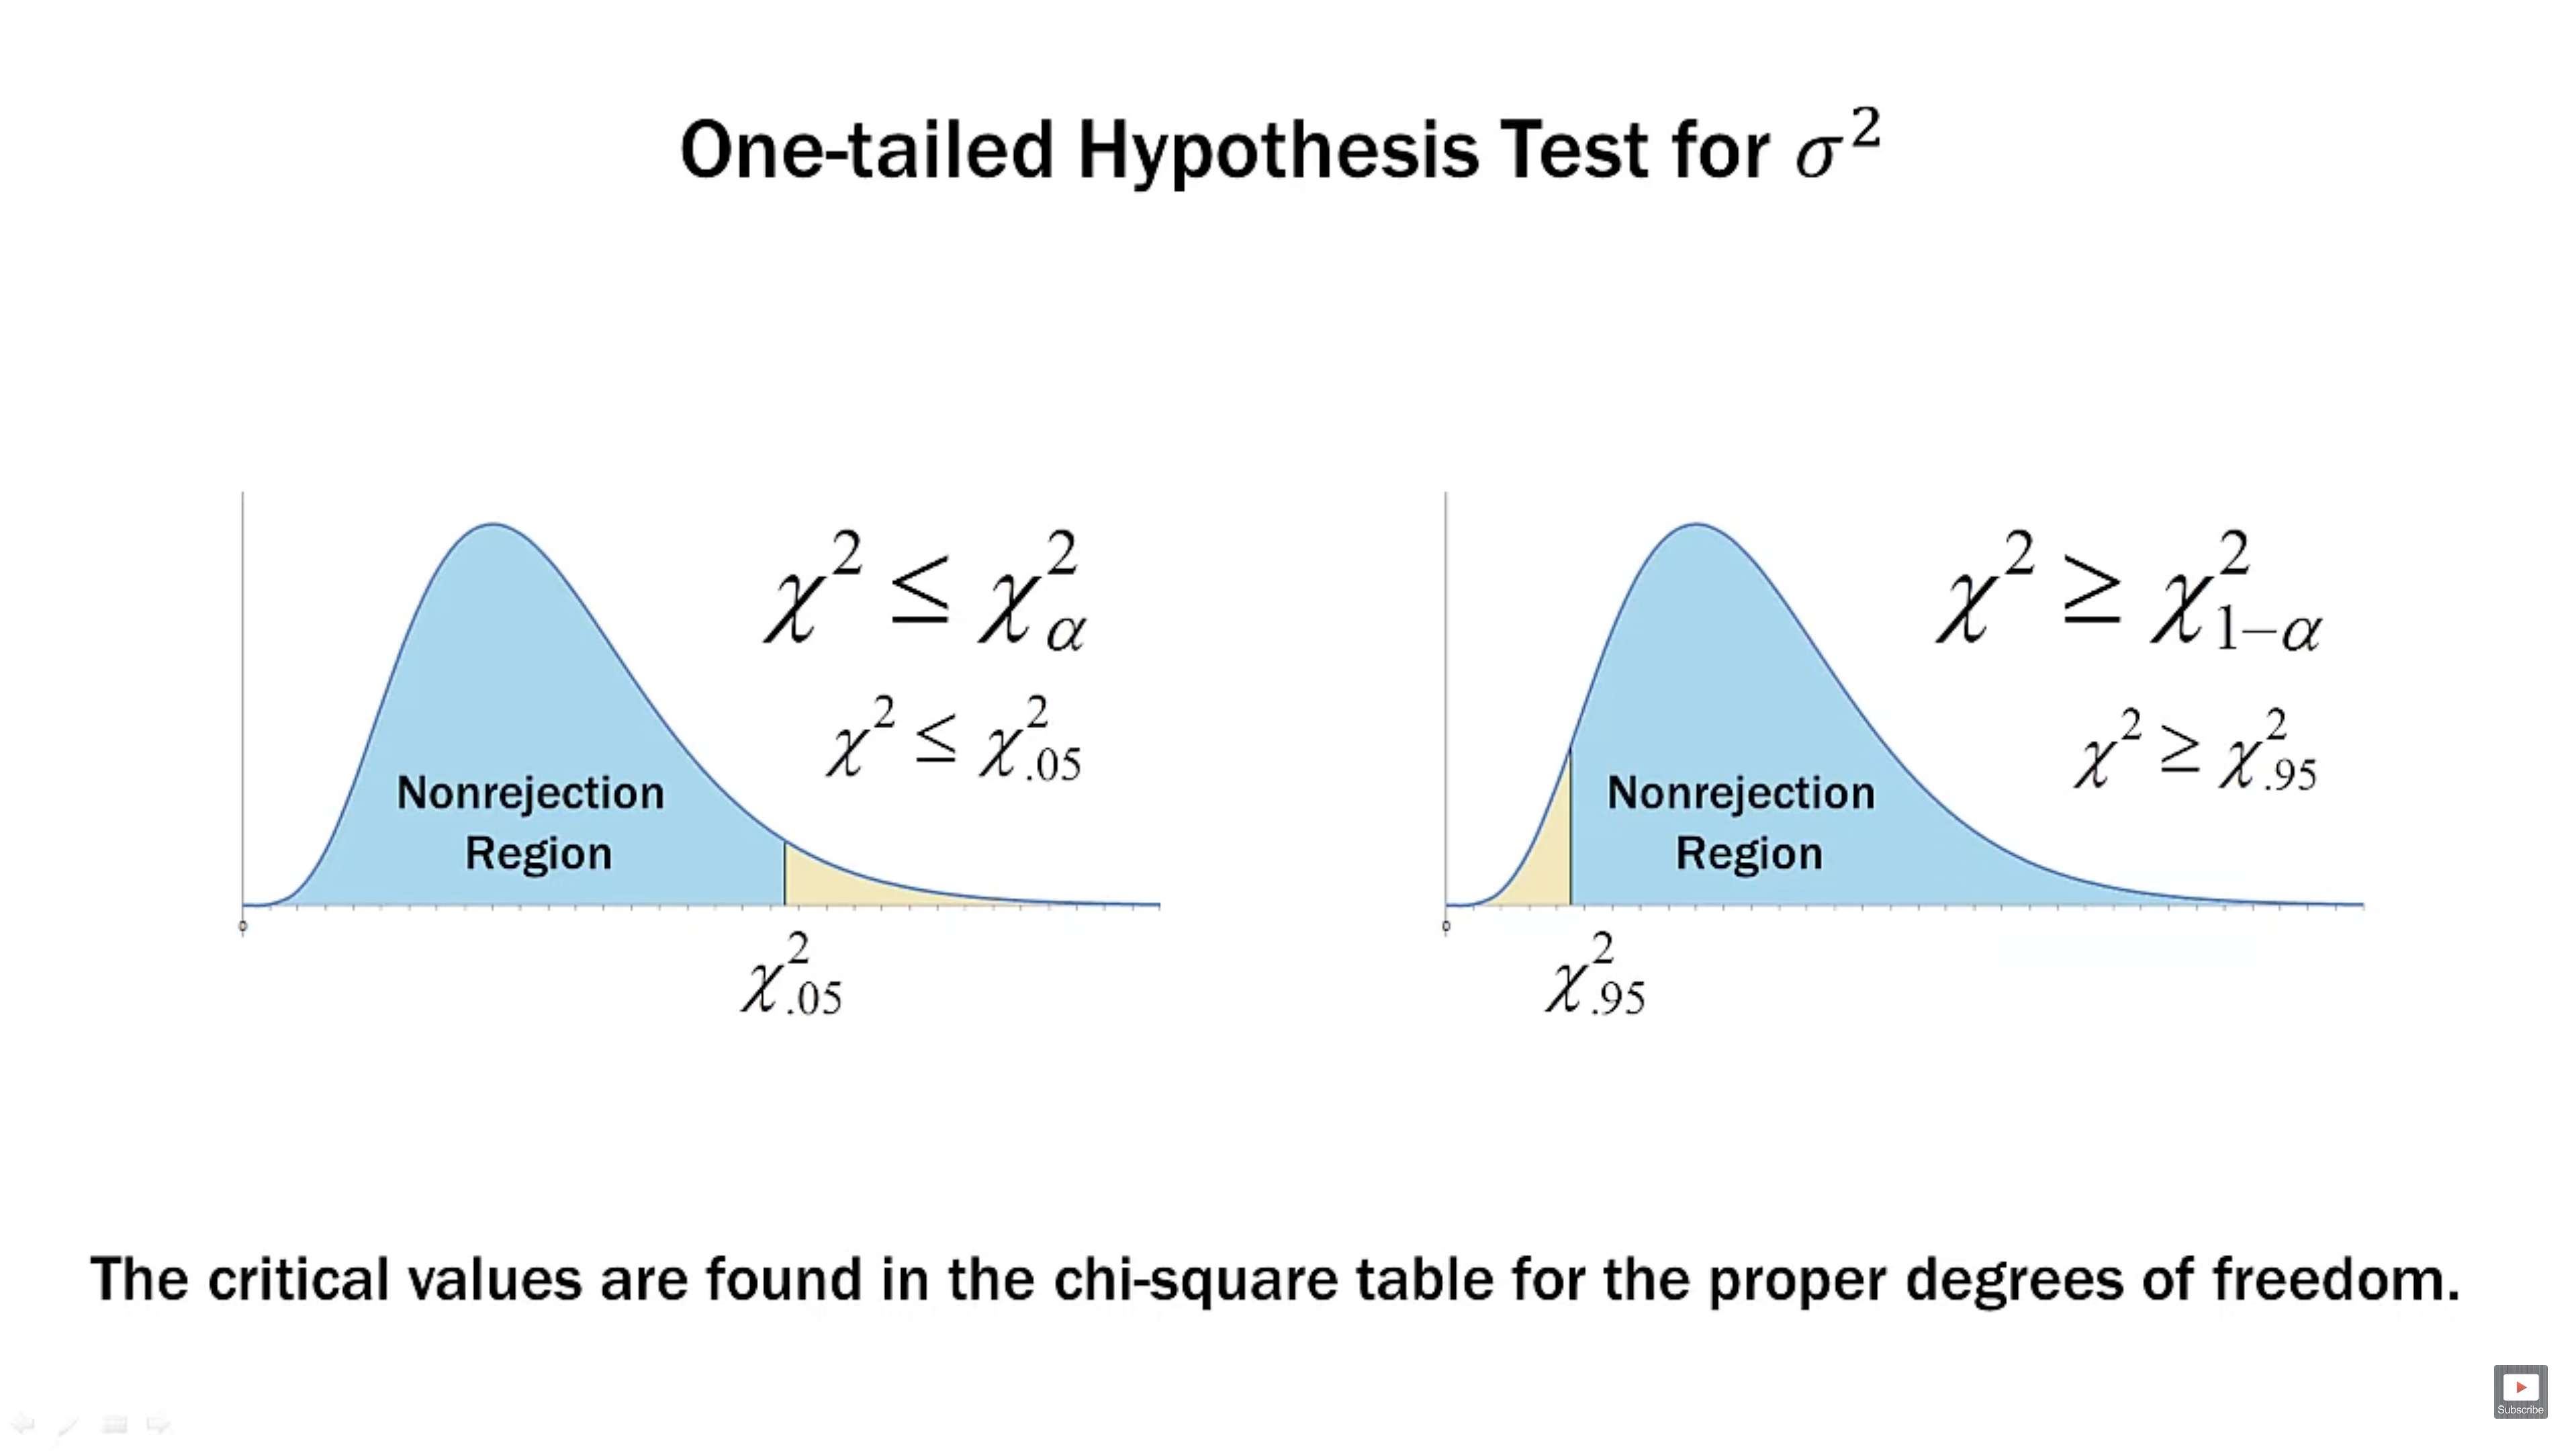
\includegraphics[width=0.45\linewidth]{varhtestonetail.png}
\end{figure}

\begin{itemize}
    \item Two-tailed: $H_0: \sigma^2 = \sigma_0^2, H_a: \sigma^2 \ne \sigma_0^2$
    \item Upper/right-tailed: $H_0: \sigma^2 \leq \sigma_0^2, H_a: \sigma^2 > \sigma_0^2$
    \item Lower/left-tailed: $H_0: \sigma^2 \geq \sigma_0^2, H_a: \sigma^2 < \sigma_0^2$
    \item Very similar to other tests, but of course, use $\chi^2$ instead of normal distribution
    \item $\chi^2=\frac{(n-1)s^2}{\sigma^2}$
\end{itemize}

\subsection{$F$-distribution for Two Samples}

\begin{figure}[H]
    \centering
    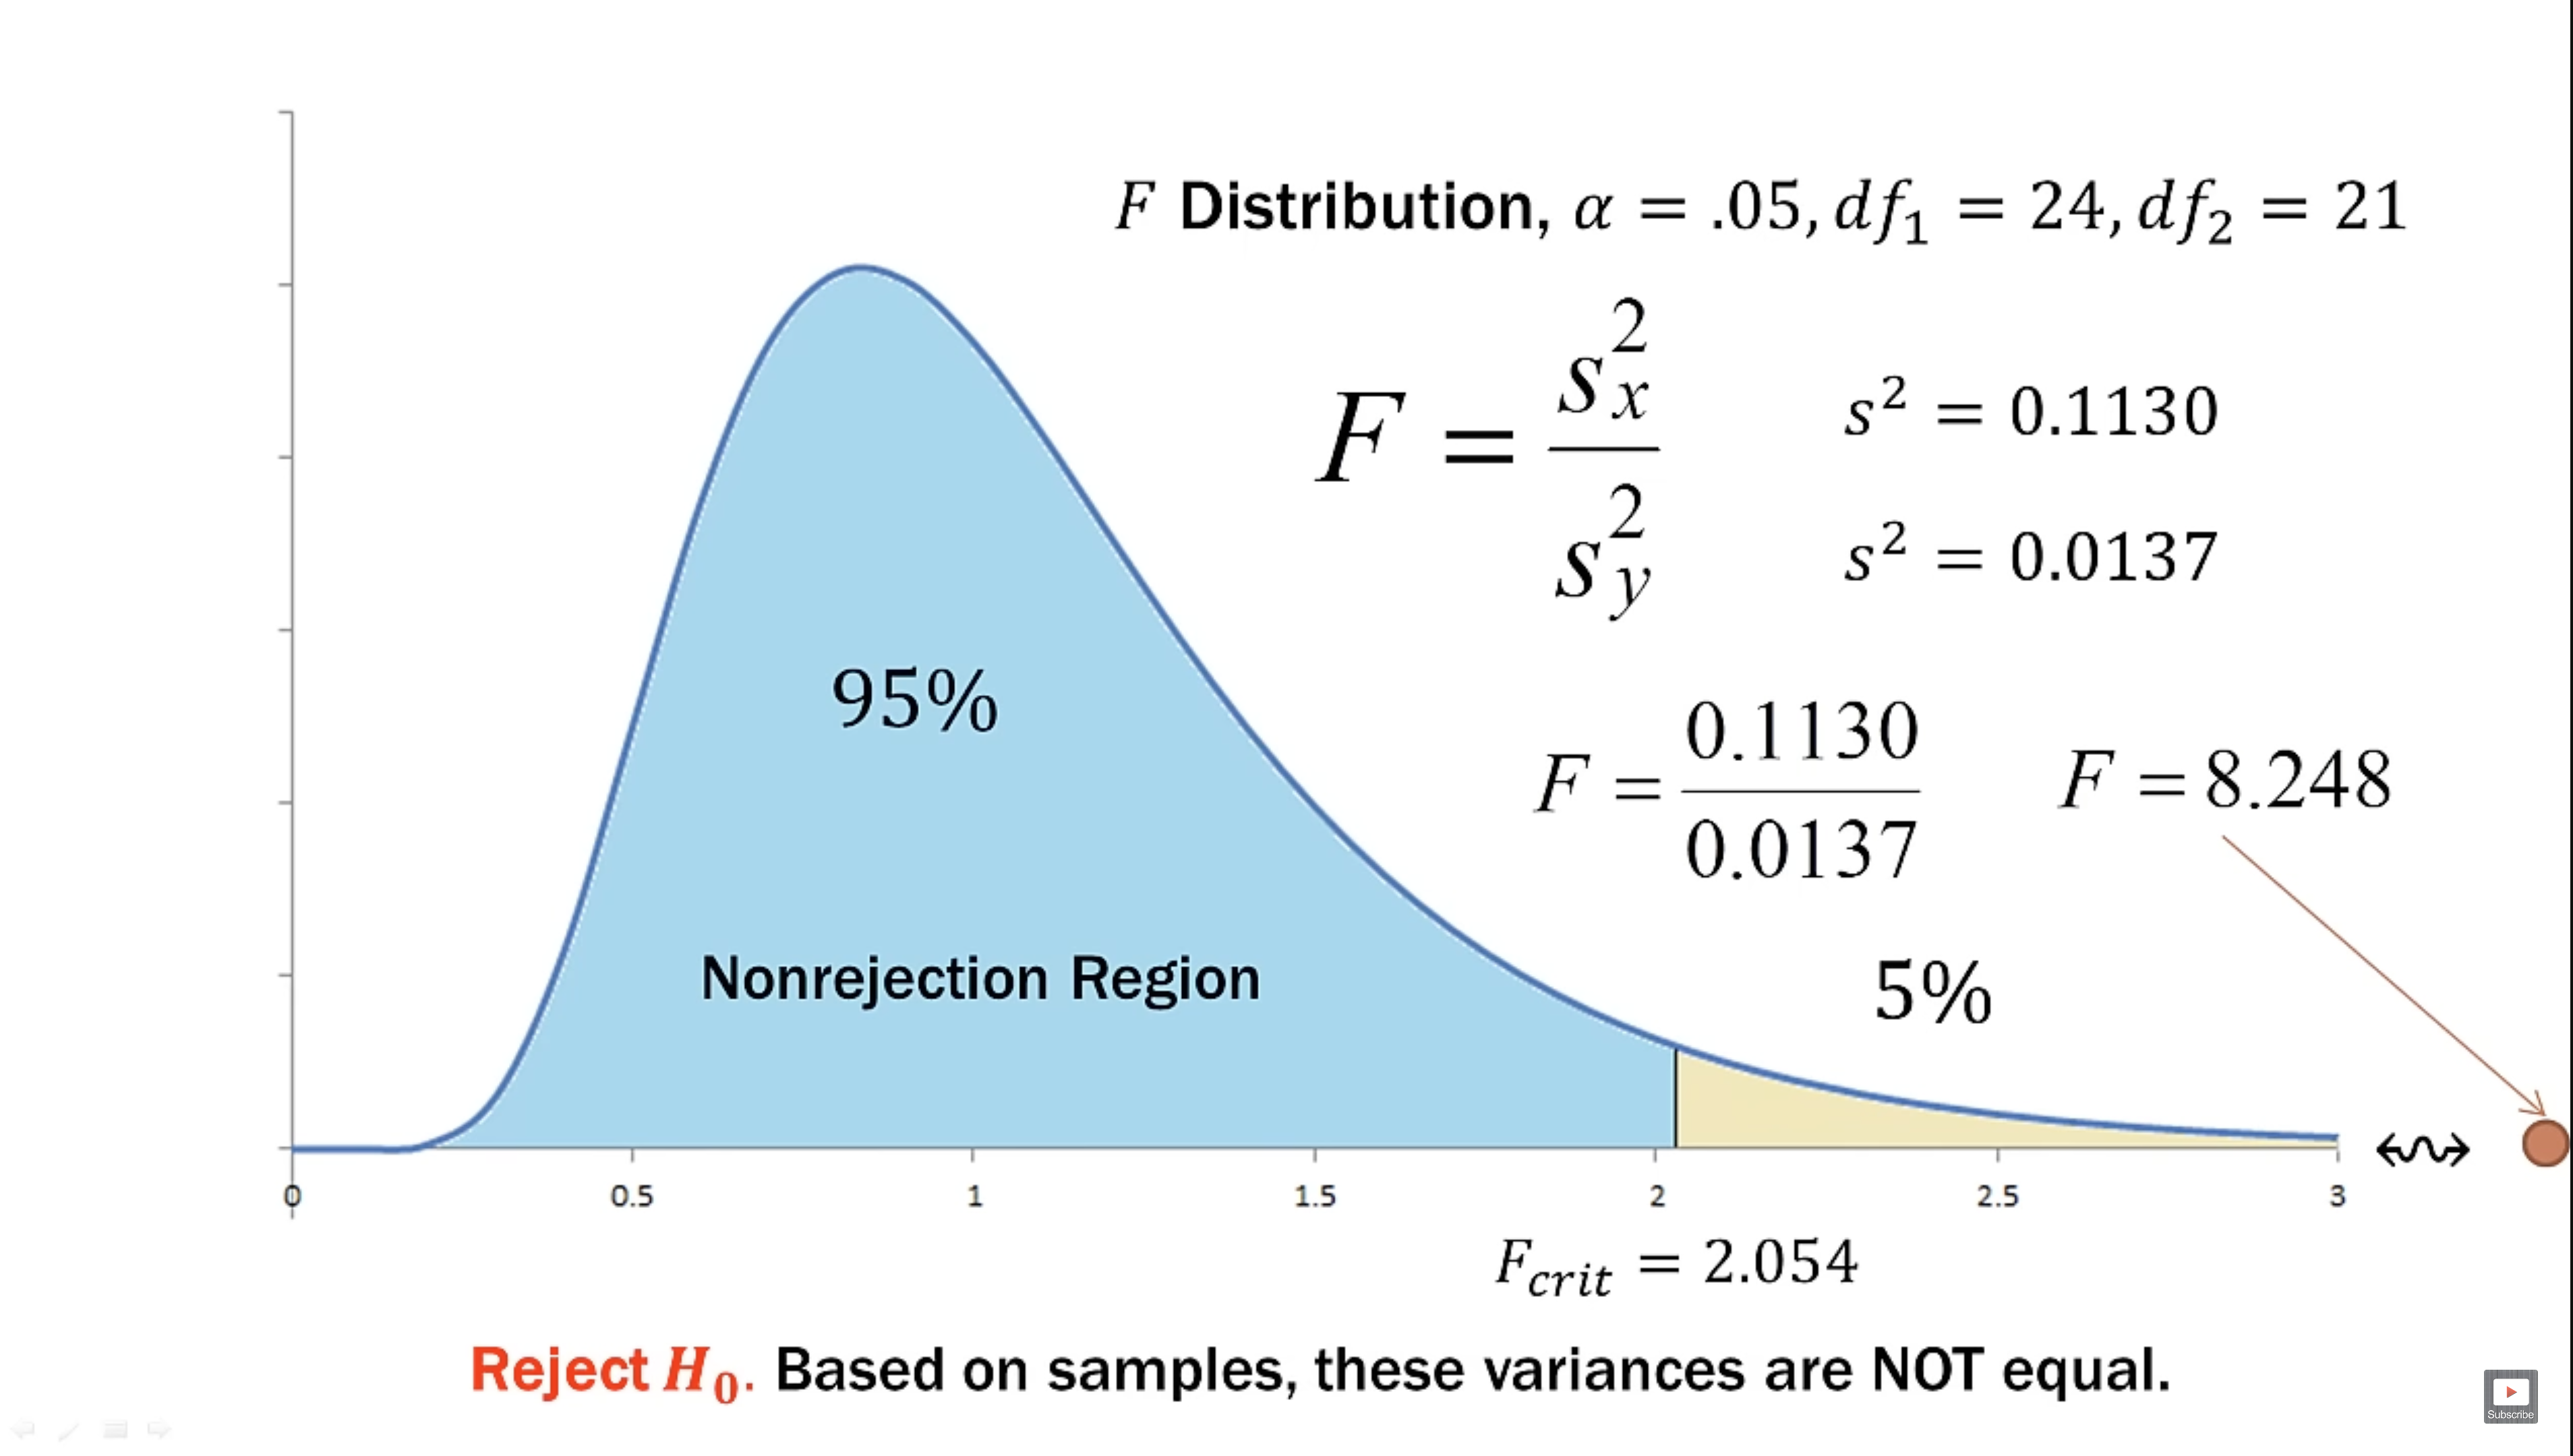
\includegraphics[width=1.0\linewidth]{ftestexample.png}
\end{figure}

\begin{itemize}
    \item Used for comparing two sample variances with each other
    \item \textbf{F-ratio}: $F=\frac{s_x^2}{s_y^2}$
    \begin{itemize}
        \item $s_x^2=\text{larger sample variance}$
        \item $s_y^2=\text{smaller sample variance}$
    \end{itemize}
    \item When independent random samples, $n_x$ and $n_y$, and are taken from two normal populations with equal variances, the sampling distribution of the ratio of those sample variances follows the $F$-distribution 
    \item The F-distribution is a distribution of ratios
    \item In the numerator, it has $n_x-1$ df, while in the denominator it has $n_y-1$ df
    \item $F$-distribution table has numerator df as columns, denominator df as rows
    \item \textbf{Hypothesis tests for variances}:
    \begin{itemize}
        \item $H_0: \sigma_x^2=\sigma_y^2, H_a: \sigma_x^2\ne \sigma_y^2$ (upper/right-tailed)
        \item Not two-tailed (even though $=$) because the numerator is always the bigger
        \item If the test statistic is larger than the critical $F$-value, reject the null hypothesis
    \end{itemize}
\end{itemize}

\section{ANOVA}

\begin{itemize}
    \item ANOVA: ANalysis Of VAriance
    \item Variability between distributions - distance of each mean from overall population mean
    \item Variability within distributions - variance/spread of each distribution
    \item ANOVA is a variability ratio $= \frac{\text{variability between}}{\text{variability within}}$
    \item When ratio is:
    \begin{itemize}
        \item $\frac{\text{LARGE}}{\text{small}}=\text{Reject} H_0$, at least one mean is an outlier and each distribution is narrow; distinct from each other
        \item $\frac{\text{similar}}{\text{similar}}=\text{Fail to reject} H_0$, means are fairly close to overall mean and/or distributions overlap a bit
        \item $\frac{\text{small}}{\text{LARGE}}=\text{Fail to reject} H_0$, means are very close to overall mean and/or distributions "melt" together
    \end{itemize}
    \item For a group $j$:
    \begin{itemize}
        \item $\bar{y_j}=\frac{1}{n_j} \sum_{i:g(i)=j} y_i$
        \item $s_j=\frac{1}{n_j-1} \sum_{i:g(i)=j} (y_i - \bar{y_j})^2$
        \item And pooled within-group std dev is: $s=\sqrt{\frac{1}{n-k} \sum_{j=1}^k (n_j-1)s_j^2}$
    \end{itemize}
\end{itemize}

\subsection{One-way ANOVA}

\begin{itemize}
    \item Suppose we want to compare $k$ population means to see if they all come from a common population, or if some means are so far away from the others it's likely they're not from the same population
    \item We have $k$ different columns/groups, with random samples within each group
    \item Each group will have it's own mean, and an overall mean
    \item The model assumes $k$ different groups, and $g(i)$ denotes the group of observation $i$
    \item Technically, the model refers to: $y_i=\mu_{g(i)}+\epsilon_i, i=1,2,...,n$
    \item Sum of squares $SS=\text{sum of square distances to mean}=\sum_{i=0}^{n}(x_i-\mu)^2$
    \item In One-Way ANOVA:
    \begin{itemize}
        \item $\text{SST}=\text{SS}=\text{SSC}+\text{SSE}$: total/overall sum of squares, $df_{\text{total}}=n-1=df_{\text{SSC}}+df_{\text{SSE}}$
        \item $\text{SSC}=\sum_{j=0}^{k}(\bar{x}_j-\mu)^2$: sum of squares between groups (columns), $df_{\text{groups}}=k-1$
        \item In course $\text{SSC}$ is called $\text{SSG}$ or $\text{SS}_{\text{grp}}$
        \item $\text{MSC}=\frac{\text{SSC}}{df_{\text{groups}}}$
        \item $\text{SSE}=\sum_{i=0}^{n}(x_i-\bar{x}_{g(i)})^2$: sum of squares within groups, $df_{\text{error}}=n-k$
        \item $\text{MSE}=\frac{\text{SSE}}{df_{\text{error}}}$
        \item $F=\frac{\text{MSC}}{\text{MSE}}$, $F=\frac{df=k-1}{df=n-k}$
        \item If the $F$-statistic is higher than our critical $F$-value, we reject $H_0$; otherwise, we fail to reject $H_0$
    \end{itemize}
    \item All these formulas also work with $y$ notation (remember in ANOVA there's just one, not $x$ and $y$, it's simply a matter of notation), but obviously replace $\mu$ with $\bar{y}$, so for example:
    \begin{itemize}
        \item $\text{SSE}=\sum_{i=1}^{n} (y_i-\bar{y_{g(i)}})^2$
        \item $\text{SSC}=\sum_{j=1}^k n_j(\bar{y_j}-\bar{y})^2$
        \item $\text{SST}=\sum_{i=1}^n (y_i -\bar{y})^2$
    \end{itemize}
    \item Residuals: $r_i=\text{observation}-\text{estimate}=y_i-\bar{y_g(i)}$
    \item Residual sum of squares: $\sum_{i=1}^{n} r_i^2=\sum_{i=1}^{n}(y_i-\bar{y_{g(i)}})^2=\text{SSE}$
    \item The pooled standard deviation can be obtained from the residual sum of squares: $s=\sqrt{\frac{1}{df} \sum_{i=0}^{n} r_i^2}$
\end{itemize}

\subsection{Two-way ANOVA without replication}

\begin{itemize}
    \item Also known as randomized block design
    \item In One-Way ANOVA, we selected a random sample for each column/group
    \item A Two-Way ANOVA allows us to "account for variation" at the row level due to some other factor/grouping
    \item By adding blocks or factors to the rows, we can "subtract out" that row variance from the overall error variance
    \item This allows greater focus on column/group differences making it easier to detect group differences
    \item Essentially, we are attempting to minimize the error variance by assigning some of it to the rows
    \item In Two-Way ANOVA, there are 4 types of sum of squares/sources of variance: 
    \begin{itemize}
        \item Total
        \item Columns/groups (between group)
        \item Rows/blocks
        \item Error (within group)
    \end{itemize}
    \item Called "without replication" because each row/block is sampling in each column/group once (one sample per cell) - randomized because order is random, each block won't necessarily sample in each group in the same order
    \item Instead of there just being the overall mean and column means $\bar{x_{C(c)}}$, there are also row means $\bar{x_{R(r)}}$, where $c$ is the number of groups/columns and $r$ is the number of rows/blocks
    \item We split $\text{SSE}$ into $\text{SSB}$ (between block variance) and $\text{SSE}$, for two-way: $df_{\text{error}}=(C-1)(R-1)$
    \item $\text{SSB}=\sum_{r=0}^{R}(\bar{x}_{R(r)}-\mu)^2$: sum of squares between blocks (rows), $df_{\text{blocks}}=R-1$
    \item $\text{MSB}=\frac{\text{SSB}}{df_{\text{blocks}}}$
    \item $\text{SST}=\text{SSC}+\text{SSB}+\text{SSE}$, if we find 3 we can solve for the fourth
    \item In two-way, you also have $F_{blocks}=\frac{\text{MSB}}{\text{MSE}}$, in addition to $F_{groups}=\frac{\text{MSC}}{\text{MSE}}$
\end{itemize}

\subsection{Two-way ANOVA with replication}

\begin{itemize}
    \item Blocks (rows) can have replication, thus each cell can have it's own mean and variance
    \item Replication means that each block has multiple number of measurements (equal amount in each block)
    \item An interaction occurs when the effect of one factor changes for different levels of the other factor
    \begin{itemize}
        \item On a marginal means graph, we look to see if the row lines cross or would cross
        \item If the interaction is significant, the row/column factors' significance can't be analyzed; the factors are too intertwined
        \item Marginal means graph = scatter/line plot of row means (line for each block) with groups (columns) on x axis
        \item Row means spread far apart from the overall mean indicate a significant row factor
    \end{itemize}
    \item Hand calculation for this is lengthy, one would typically use R (or other tools) for this
\end{itemize}

\subsection{Post Hoc Test (Fisher's LSD)}

\begin{itemize}
    \item ANOVA only tells us if the population means are equal; if the $F$-test is significant, we do not know where the differences are located
    \item Thus, it is necessary to compare each population post hoc (after the fact), with $k \text{choose} 2$ for $k$ groups
    \item In Fisher's test:
    \begin{itemize}
        \item $H_0: \mu_i = \mu_j$ for a pair of groups $i$ and $j$
        \item $H_1: \mu_i \ne \mu_j$ 
        \item $t = \frac{\bar{x_i}-\bar{x_j}}{\sqrt{\text{MSE} \cdot (\frac{1}{n_i} + \frac{1}{n_j})}}$
        \item For $t$-test, df:$n-k$
        \item $\text{LSD}=t_{\alpha/2}\sqrt{\text{MSE} \cdot (\frac{1}{n_i} + \frac{1}{n_j})}$
        \item Reject $H_0$ if $|\bar{x_i} - \bar{x_j}|\geq \text{LSD}$
    \end{itemize}
\end{itemize}

\section{Simple Linear Regression}

Key steps:
\begin{enumerate}
    \item Use least-squares to fit a line to the data
    \item Calculate $r^2$
    \item Calculate a $p$-value for $r^2$
\end{enumerate}

\subsection{Residuals}

\begin{itemize}
    \item Residuals are the differences between the observed and predicted values
    \item For a best fit line, the residuals (non square) should add up to 0
    \item In the least squares method, coefficients for the regression are found such that they minimize the sum of squares of the residuals $=\text{Sum of squared errors}=\text{SSE}$
    \item The goal of simple linear regression is to create a linear model that minimizes the sum of squares of the residuals/error ($\text{SSE}$)
    \item We denote the standard deviation of the residuals as $s_{y|x}=\sqrt{\frac{\sum_{i=0}^n r_i^2}{n-2}}$
\end{itemize}

\subsection{Model}

\begin{itemize}
    \item In a linear model, the value of the dependent variable $y$ is a function of the independent variable $x$
    \item $y=\beta_0 + \beta_1 x + \epsilon$, where $\epsilon$ is the error term: unexplained variation in $y$
    \item In a regression equation, we write $E(y)=\beta_0 + \beta_1 x$
    \item Technically, $E(y)$ isn't a point, but the mean of the distribution of $y$ values for that $x_i$: $Y_i \sim N(\beta_0 + \beta_ 1 x_i, \sigma^2)$
    \item When using sample data, $\hat{y}=b_0+b_1 x$, where $\hat{y}$ is the point estimator of $E(y)$ - the mean value of $y$ for a given value for $x$
\end{itemize}

\subsection{Least Squares Method}

\begin{itemize}
    \item Least squares criterion: $\min \sum_{i=0}^{n}(y_i - \hat{y_i})^2$, where $y_i$ is the observed value, and $\hat{y_i}$ is the predicted value
    \item Checking the correlation coefficient $r$ can be a good indicator for if there's a strong linear relationship suitable for linear regression
    \item Centroid is at $(\bar{x},\bar{y})$ (mean $x$/$y$ value); the best-fit regression line will pass through the centroid
    \item $b_1=\hat{\beta_1}=\frac{\sum_{i=0}^{n}(x_i-\bar{x})(y_i-\bar{y})}{\sum_{i=0}^{n}(x_i-\bar{x})^2}$
    \item Alternatively, $b_1=\frac{n\sum(x_i y_i)-(\sum x_i)(\sum y_i)}{n \sum (x_i^2)-(\sum x_i)^2}$
    \item $b_0=\bar{y}-b_1\bar{x}$
    \item For variance, an unbiased estimator is: $\hat{\sigma^2}=\frac{1}{n-2} \sum_{i=1}^n (Y_i-b_0-b_1x_i)^2$
\end{itemize}

\subsection{Fit}

\begin{itemize}
    \item It's improper to use a model to extrapolate from outside the bounds of the data it was calculated from
    \item The difference between $\text{SST}$ and $\text{SSE}$ is due to regression, $\text{SSR}$ (reminder: $\text{SST}$ is the sum of squares between $y_i$ and $\bar{y}$, while $\text{SSE}$ is the sum of squares between observed and predicted $y$ values). $\text{SSR}=\text{SST}-\text{SSE}$
    \item $\text{Var}(\text{fit})=\frac{\text{SSE}}{n}$
    \item \textbf{Coefficient of Determination}:
    \begin{itemize}
        \item How well does the estimated regression fit our data?
        \item We partition $SST$ into $SSR$ and $SSE$, if the $SSR$ is large, it uses up more of the $SST$ and therefor $SSE$ is smaller
        \item The coefficient of determination quantifies this ratio as a percentage
        \item $r^2=\frac{\text{SSR}}{\text{SST}}$
        \item It means that $r^2$\% of the total sum of squares can be explained using the estimated regression equation
        \item Alternatively, we can say that the independent variable "explains" $r^2$\% of the variation in the dependent variable
    \end{itemize}
\end{itemize}

\begin{figure}[H]
    \centering
    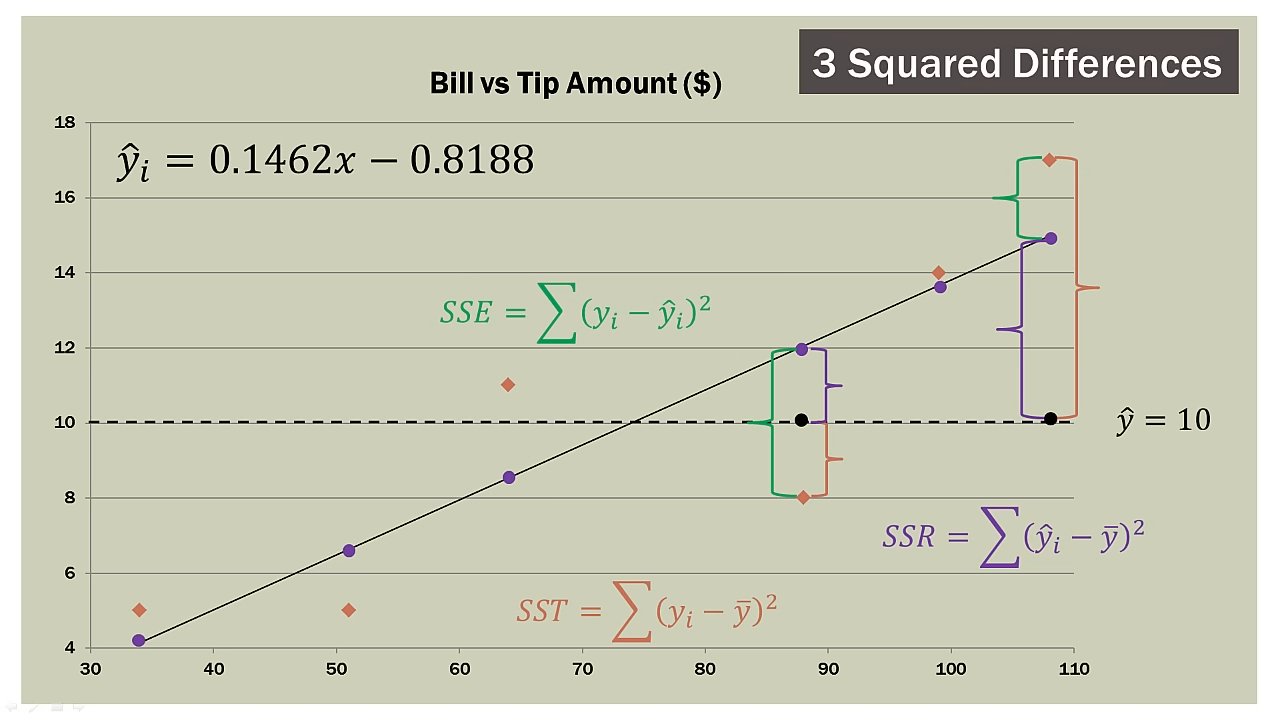
\includegraphics[width=0.5\linewidth]{sse_sst_ssr.jpeg}
\end{figure}

\subsubsection{\( p \)-value}

\begin{itemize}
    \item In the context of regression analysis, the \( F \)-statistic is used to test the overall significance of the model. It is calculated as:
    \[
    F = \frac{\text{MSR}}{\text{MSE}}
    \]
    where \(\text{MSR} = \frac{\text{SSR}}{p}\) is the mean square regression and \(\text{MSE} = \frac{\text{SSE}}{n - p - 1}\) is the mean square error. Here, \( p \) is the number of predictors and \( n \) is the total number of observations ($p$ is $1$ for simple linear regression)
    \item The \( F \)-statistic follows an \( F \)-distribution with \( p \) and \( n - p - 1 \) degrees of freedom
    \item To test the null hypothesis \( H_0: \beta_1 = \beta_2 = \cdots = \beta_p = 0 \) (no linear relationship), we compare the calculated \( F \)-value to the critical value from the \( F \)-distribution table at a given significance level (e.g., \(\alpha = 0.05\)). If the \( F \)-value is greater than the critical value, we reject the null hypothesis
    \item The $p$-value associated with the $F$-statistic indicates the probability of observing such an $F$-value if $H_0$ is true. A smaller $p$-value suggests that the model provides a better fit than would be expected by chance
\end{itemize}

\subsection{Standardized Regression}

\begin{itemize}
    \item Useful for interpreting variables having very different scales and variances
    \item In multiple regression helps determine which variables account for the most variance in the dependent variable
    \item $z_{xi}=\frac{x_i-\bar{x}}{s_x}$
    \item $z_{yi}=\frac{y_i-\bar{y}}{s_y}$
    \item We can plot these standardized values $(z_{xi}, z_{yi})$
    \item Correlation in standardized data is the same as raw data
    \item Centroid of standardized data is $(0,0)$
    \item $y=rx$, so the intercept is at $0$, and the slope is the correlation $r$
    \item The original regression slope for the raw data $=r \cdot \frac{s_y}{s_x}$
    \item Thus, $r=b_1 \cdot \frac{s_y}{s_x}$
\end{itemize}

\subsection{Model Error}

\begin{itemize}
    \item $\text{SSE}=\sum_{i=0}^{n}(y_i-\hat{y_i})^2$
    \item MSE $s^2$ is an estimate of $\sigma^2$, the variance of the error $\epsilon$; $s^2=\text{MSE}=\frac{\text{SSE}}{n-2}$
    \item $s=\sqrt{MSE}$ is the average distance of the data points from the regression line, it can be used to make prediction intervals
    \item Root Mean Square Error $s$ (standard error) shows how well the data points fit around a regression line
    \item $r^2=\frac{\text{SSR}}{\text{SST}}$
\end{itemize}

\subsection{Confidence Interval for the Slope}

\begin{itemize}
    \item $=b_1\pm t_{\alpha/2} \cdot s_{b1}$
    \item $s_{b1}=\frac{s}{\sqrt{\sum_{i=0}^n(x_i-\bar{x})^2}}$
    \item $t$-value df:$n-2$
    \item $H_0: \beta_1=0, H_a: \beta_1 \ne 0$
    \item If the confidence interval does not contain zero, we reject $H_0$
    \item Alternatively, test statistic $t=\frac{b_1}{s_{b1}}$
\end{itemize}

\subsection{Confidence Interval Bands}

\begin{itemize}
    \item The mean value of $\hat{y}$ for any $x$ has a confidence interval
    \item Not to be confused with prediction intervals, for an individual $\hat{y}$ of a value of $x$
    \item The confidence interval is for the mean value, not individual value; it captures the uncertainty around the mean predicted values
    \item $x^*=$ the value of interest for the dependent variable $x$
    \item $y^*=$ the possible values $y$ may take when $x=x^*$
    \item $E(y^*)=$ the expected value or mean of $y$ when $x=x^*$
    \item $\hat{y^*}=b_0+b_1x^*$
    \item $\hat{y^*} \pm t_{\alpha/2} s_{\hat{y^*}}$, df:$n-2$
    \item $s_{\hat{y^*}}=s \sqrt{\frac{1}{n}+\frac{(x^*-\bar{x})^2}{\sum_{i=0}^{n}(x_i-\bar{x})^2}}$
    \item The most precise estimate of the mean value of $y$ is when $x^*=\bar{x}$, as $x^*$ gets further from $\bar{x}$ the confidence interval will become wider, and the confidence band will flare out towards the tips
    \item For linear regression, can be written as $=\hat{\beta_0}+\hat{\beta_1} \cdot x_0 \pm t_{\alpha/2,n-2} \cdot s \cdot \sqrt{\frac{1}{n}+\frac{(x_0-\bar{x})^2}{\sum (x_i-\bar{x})^2}}$
\end{itemize}

\subsection{Prediction Interval Bands}

\begin{itemize}
    \item The prediction interval will always be wider than the confidence interval
    \item A $p$\% prediction interval is an interval that has a $p$\% probability of containing a new observation
    \item A prediction interval captures uncertainty around a single value
    \item $\hat{y^*} \pm t_{\alpha/2} s_{\text{pred}}$
    \item $s^2_{\text{pred}}=s^2+s^2_{\hat{y^*}}$
    \item Just like with confidence interval bands, most precise when $x^*=\bar{x}$, flares out towards tips
    \item For linear regression, can be written as $=\hat{\beta_0}+\hat{\beta_1} \cdot x_0 \pm t_{\alpha/2,n-2} \cdot s \cdot \sqrt{1+\frac{1}{n}+\frac{(x_0-\bar{x})^2}{\sum (x_i-\bar{x})^2}}$
\end{itemize}

\subsection{Residual Analysis}

\begin{itemize}
    \item A residual is a quantity remaining after other things have been subtracted or accounted for
    \item The difference between the observed value and what is predicted by the regression model
    \item $=y_i-\hat{y_i}$
    \item Only part of the variance in the dependent variable will be explained by the values of the independent variable; $r^2$, ($\frac{\text{SSR}}{\text{SST}}$)
    \item The variance left unexplained is due to model error ($\frac{\text{SSE}}{\text{SST}}$)
    \item Residuals offer the best information about the error term, $\epsilon$
    \item The expected value of the error term is zero; $E(\epsilon)=0$
    \item For all values of the independent variable $x$, the variance of the error term $\epsilon$ is the same
    \item The values of the error term $\epsilon$ are independent of each other
    \item The error term $\epsilon$ follows a normal distribution
    \item We can scatter plot residuals against both $x$ and $y$
    \item If the residuals are randomly scattered, we call it homoscedasticy (constant variance)
    \item However, if we have heteroscedasticity (non-constant variance), that indicates a problem with the model, such as non-linear data
\end{itemize}

\subsection{Outliers and Influential Observations}

\begin{itemize}
    \item Scatter plots are a great way to spot outliers
    \item An outlier can influence the regression line "pulling" it in the direction of the outlier
    \item An influential observation may be an outlier, but not necessarily. It could also be a value that is far outside the rest of the values for the data. It can also influence the model significantly.
    \item Sometimes they can be caused by observational errors, while other times they are genuine and may suggest a different non-linear model should be used. Sometimes they are just extreme values that are in the dataset by random chance.
    \item Leverage of data point $i$: $h_i=\frac{1}{n} + \frac{(x_i-\bar{x})^2}{\sum_{j=0}^n(x_j-\bar{x})^2}$
    \item Where $p$ is the number of independent variables: $h_i>\frac{3(p+1)}{m}$ is the decision value. If $h_i>\text{decision value}$, then that value has a large influence on the simple regression analysis
\end{itemize}

\subsection{Design Matrices}

\begin{itemize}
    \item A design matrix isn't always a bunch of 0's and 1's, but can be any set of numbers or variables that we want to plug into an equation, one row at a time
\end{itemize}

\subsection{Linear transformations}

\begin{itemize}
    \item $E(aX+b)=aE(X)+b$
    \item $\text{Var}(aX+b)=a^2 \text{Var}(X)$
    \item $\text{Cov}(aX_1+b,cX_2+d)=ac \text{Cov}(X_1,X_2)$
\end{itemize}

\section{Multiple Linear Regression}

\begin{itemize}
    \item Adding more independent variables does not mean the regression will be "better" - be careful of overfitting
    \item Independent variables can be related to each other, when this happens, it's called multicollinearity
    \item Ideally, each independent variable is correlated with the dependent variable but not with each other
    \item \textbf{Multiple Regression Model}: $y=\beta_0 + \beta_1 x_1 + \beta_2 x_2 + \dots + \beta_p x_p + \epsilon$
    \item \textbf{Multiple Regression Equation}: $E(y)=\beta_0 + \beta_1 x_1 + \beta_2 x_2 + \dots + \beta_p x_p$
    \item \textbf{Estimated Multiple Regression Equation}: $\hat{y}=b_0 + b_1 x_1 + b_2 x_2 + \dots + b_p x_p$
    \item In multiple regression, each coefficient is interpreted as the estimated change in $y$ corresponding to a one unit change in a variable, when all other variables are held constant
    \item For a multiple regression model, $\text{MSE}=\frac{\text{SSE}}{df_e}=\frac{\sum_{i=0}^{n}(y_i-\hat{y_i})^2}{n-p-1}=s_e^2$
    \item \textbf{See Week 9 slides for lots of useful info, about the matrices, least squares, MLE, etc.}
\end{itemize}

\subsection{Data Preparation}

\begin{enumerate}
    \item Check the relationships between each independent variable (feature) and the dependent variable using scatterplots and correlations - if any has low correlation, it's non-contributing, and should be excluded
    \item Check the relationships among the independent variables using scatterplots and correlations (check for multicollinearity) - if any two are highly correlated, don't use both in multiple regression; they are redundant
    \begin{itemize}
        \item VIF (variance inflation factor) assesses how much the variance of an estimated regression coefficient increases if the predictors are correlated
        \item If it's 1, no factors are correlated
        \item 5-10 indicates high correlation and may be problematic
        \item Anything above 10, the regression coefficients are poorly estimated due to multicollinearity
    \end{itemize}
    \item Use non-redundant independent variables to find the best fitting model
    \item Remember, $\text{SST}$ is split into $\text{SSR}$ and $\text{SSE}$, and $r^2=\frac{\text{SSR}}{\text{SST}}$
    \item The goal is to maximize $\text{SSR}$ and minimize $\text{SSE}$ as a proportion of the $\text{SST}$, but not at the cost of overfitting
    \item \textbf{F-Test for Feature Decision}: $F=\frac{\frac{\text{SSE}_{\text{fewer features}}-\text{SSE}_{\text{more features}}}{\text{num features added}}}{\text{MSE}_{\text{more features}}}$, df:$\frac{\text{num features added}}{\text{df for MSE}_{\text{more features}}}$ - this is just a test, do not rely blindly on it, but it can be used to filter out non-contributing features
\end{enumerate}

\subsection{Dummy Variables}

\begin{itemize}
    \item Dummy variables let us use categorical variables in our regression
    \item For $k$ categories/groups, we have $k-1$ dummy variables
    \item We have dummy variables $x_1,\dots,x_{k-1}$
    \item $x_i=1$ for category $i$ and every other dummy is 0
    \item For the $k$-th category, we code it with 0's for all dummy variables (think of it as the "default" category, who's effect on $y$ is encoded in the constant term $\beta_0$, while each dummy variable accounts for $\beta_0$'s value)
    \item When we have two (or more) categorical variables, nothing changes. Each one will just add $k-1$ dummy variables
\end{itemize}

\subsection{Adjusted $R^2$}

\begin{itemize}
    \item Adjusted $R^2$ penalty - a balance between the number of feature variables and the number of observations
    \item Most severe adjustment made on models that have many features relative to the number of observations
    \item $R_a^2=R^2-\frac{p(1-R^2)}{n-p-1}$, where $n$ is the number of observations and $p$ the number of features
    \item Alternatively, $R_a^2=1-(\frac{n-1}{\text{SST}}) \cdot \text{MSE}$
\end{itemize}

\subsection{Linear transformations}

\begin{itemize}
    \item $E(AX+b)=AE(X)+b$
    \item $\text{Var}(AX+b)=A\text{Var}(X)A^T$
\end{itemize}

\subsection{Design Matrix for Multiple Regression}

\begin{itemize}
    \item The design matrix $X$ for multiple regression includes a column of ones (for the intercept term) and columns for each independent variable.
    \item $X$ has the following properties:
    \begin{itemize}
        \item $X$ is deterministic
        \item $X$ has full rank, $\text{rank}(X)=p, p<n$
        \item $\epsilon \sim N(0,\sigma^2\textbf{I})$
        \begin{itemize}
            \item Mean of errors $=0$
            \item Errors homoscedastic
            \item Errors normally distributed
        \end{itemize}
    \end{itemize}
    \item For a dataset with $n$ observations and $p$ predictors, the design matrix $X$ is an $n \times (p+1)$ matrix, where the first column consists of ones.
    \item Example: If we have three predictors $x_1$, $x_2$, and $x_3$ and $n$ observations, the design matrix $X$ is:
    \[
    X = \begin{bmatrix}
    1 & x_{11} & x_{12} & x_{13} \\
    1 & x_{21} & x_{22} & x_{23} \\
    \vdots & \vdots & \vdots & \vdots \\
    1 & x_{n1} & x_{n2} & x_{n3}
    \end{bmatrix}
    \]
    \item To predict values $\hat{y}$ given certain parameters $\hat{\beta}$, we use the matrix multiplication:
    \[
    \hat{y} = X\hat{\beta}
    \]
    where $\hat{\beta}$ is the vector of estimated coefficients:
    \[
    \hat{\beta} = \begin{bmatrix}
    \hat{\beta}_0 \\
    \hat{\beta}_1 \\
    \hat{\beta}_2 \\
    \hat{\beta}_3
    \end{bmatrix}
    \]
    \item To compute the predicted values for new observations, you construct a new design matrix $X_{\text{new}}$ for the new data and multiply it by the estimated coefficients:
    \[
    \hat{y}_{\text{new}} = X_{\text{new}} \hat{\beta}
    \]
    \item Example: If we have new data with three observations, the new design matrix $X_{\text{new}}$ might look like:
    \[
    X_{\text{new}} = \begin{bmatrix}
    1 & x_{11}^{\text{new}} & x_{12}^{\text{new}} & x_{13}^{\text{new}} \\
    1 & x_{21}^{\text{new}} & x_{22}^{\text{new}} & x_{23}^{\text{new}} \\
    1 & x_{31}^{\text{new}} & x_{32}^{\text{new}} & x_{33}^{\text{new}}
    \end{bmatrix}
    \]
    and the predicted values $\hat{y}_{\text{new}}$ are obtained by:
    \[
    \hat{y}_{\text{new}} = X_{\text{new}} \hat{\beta}
    \]
\end{itemize}


\subsection{Least Squares Method}

\begin{itemize}
    \item The least squares method aims to minimize the sum of the squared differences between the observed values and the values predicted by the model.
    \item The objective function for the least squares method is: 
    \[
    \min \sum_{i=1}^{n}(y_i - \hat{y_i})^2 = \min \sum_{i=1}^{n}(y_i - (\beta_0 + \beta_1 x_{1i} + \beta_2 x_{2i} + \dots + \beta_p x_{pi}))^2
    \]
    \item To find the estimates of the coefficients, we take partial derivatives of the objective function with respect to each $\beta_j$ and set them to zero.
    \item The normal equations derived from the least squares criterion are:
    \[
    X^TX\beta = X^Ty
    \]
    where $X$ is the design matrix, $\beta$ is the vector of coefficients, and $y$ is the vector of observed values.
    \item The solution to these equations gives the least squares estimates:
    \[
    \hat{\beta} = (X^TX)^{-1}X^Ty
    \]
    \item This provides the coefficients that minimize the sum of the squared residuals, giving the best fit line for the data.
\end{itemize}

\subsubsection{Least Squares Method on TI-84}

\begin{enumerate}
    \item Enter the design matrix $X$:
    \begin{itemize}
        \item Press \code{2nd} then \code{MATRIX}, scroll to \code{EDIT}, select \code{[A]}, and set the dimensions to $n \times (p+1)$, where $n$ is the number of observations and $p$ is the number of predictors. Enter your data into matrix \code{[A]}. Ensure the first column of \code{[A]} is filled with ones for the intercept.
    \end{itemize}
    \item Enter the response vector $y$:
    \begin{itemize}
        \item Press \code{2nd} then \code{MATRIX}, scroll to \code{EDIT}, select \code{[B]}, and set the dimensions to $n \times 1$. Enter your observed values into matrix \code{[B]}.
    \end{itemize}
    \item Calculate $X^T X$:
    \begin{itemize}
        \item Press \code{2nd} then \code{MATRIX}, select \code{[A]}, then press \code{2nd} \code{MATRIX}, scroll to \code{MATH}, select \code{T} (Transpose), and press \code{ENTER}.
        \item Multiply the transpose of \code{[A]} by \code{[A]}: Press \code{2nd} \code{MATRIX}, select \code{[A]}, press \code{*}, then press \code{2nd} \code{MATRIX}, select \code{[A]}, and press \code{ENTER}. Store the result in another matrix (e.g., \code{[C]}).
    \end{itemize}
    \item Calculate $X^T y$:
    \begin{itemize}
        \item Multiply the transpose of \code{[A]} by \code{[B]}: Press \code{2nd} \code{MATRIX}, select \code{[A]}, then press \code{2nd} \code{MATRIX}, scroll to \code{MATH}, select \code{T} (Transpose), and press \code{ENTER}.
        \item Press \code{*}, then press \code{2nd} \code{MATRIX}, select \code{[B]}, and press \code{ENTER}. Store the result in another matrix (e.g., \code{[D]}).
    \end{itemize}
    \item Calculate the inverse of $X^T X$:
    \begin{itemize}
        \item Press \code{2nd} \code{MATRIX}, select \code{[C]}, press \code{$x^{-1}$}, and press \code{ENTER}. Store the result in another matrix (e.g., \code{[E]}).
    \end{itemize}
    \item Calculate the coefficients $\hat{\beta}$:
    \begin{itemize}
        \item Multiply the inverse of \code{[C]} by \code{[D]}: Press \code{2nd} \code{MATRIX}, select \code{[E]}, press \code{*}, then press \code{2nd} \code{MATRIX}, select \code{[D]}, and press \code{ENTER}. The resulting matrix contains the coefficients $\hat{\beta}$.
    \end{itemize}
\end{enumerate}
    
\subsection{Maximum Likelihood Estimation (MLE)}

\begin{itemize}
    \item The MLE method finds the parameter values that maximize the likelihood function, which measures the probability of observing the given sample data.
    \item For multiple linear regression, the likelihood function assuming normally distributed errors is:
    \[
    L(\beta, \sigma^2) = \left( \frac{1}{2\pi\sigma^2} \right)^{n/2} \exp\left(-\frac{1}{2\sigma^2} \sum_{i=1}^{n} (y_i - \beta_0 - \beta_1 x_{1i} - \beta_2 x_{2i} - \dots - \beta_p x_{pi})^2 \right)
    \]
    \item The log-likelihood function is:
    \[
    \ell(\beta, \sigma^2) = -\frac{n}{2} \log(2\pi\sigma^2) - \frac{1}{2\sigma^2} \sum_{i=1}^{n} (y_i - \beta_0 - \beta_1 x_{1i} - \beta_2 x_{2i} - \dots - \beta_p x_{pi})^2
    \]
    \item Taking the partial derivatives of the log-likelihood function with respect to $\beta$ and $\sigma^2$ and setting them to zero, we obtain:
    \[
    \frac{\partial \ell}{\partial \beta} = \frac{1}{\sigma^2} X^T (y - X\beta) = 0 \Rightarrow \hat{\beta} = (X^TX)^{-1}X^Ty
    \]
    \[
    \frac{\partial \ell}{\partial \sigma^2} = -\frac{n}{2\sigma^2} + \frac{1}{2\sigma^4} \sum_{i=1}^{n} (y_i - X\beta)^2 = 0 \Rightarrow \hat{\sigma^2} = \frac{1}{n} \sum_{i=1}^{n} (y_i - X\hat{\beta})^2
    \]
    \item These estimates maximize the likelihood function, providing the best fit for the regression model.
\end{itemize}

\subsubsection{MLE on TI-84}

\begin{enumerate}
    \item Enter the design matrix $X$:
    \begin{itemize}
        \item Press \code{2nd} then \code{MATRIX}, scroll to \code{EDIT}, select \code{[A]}, and set the dimensions to $n \times (p+1)$, where $n$ is the number of observations and $p$ is the number of predictors. Enter your data into matrix \code{[A]}. Ensure the first column of \code{[A]} is filled with ones for the intercept.
    \end{itemize}
    \item Enter the response vector $y$:
    \begin{itemize}
        \item Press \code{2nd} then \code{MATRIX}, scroll to \code{EDIT}, select \code{[B]}, and set the dimensions to $n \times 1$. Enter your observed values into matrix \code{[B]}.
    \end{itemize}
    \item Calculate $X^T X$:
    \begin{itemize}
        \item Press \code{2nd} then \code{MATRIX}, select \code{[A]}, then press \code{2nd} \code{MATRIX}, scroll to \code{MATH}, select \code{T} (Transpose), and press \code{ENTER}.
        \item Multiply the transpose of \code{[A]} by \code{[A]}: Press \code{2nd} \code{MATRIX}, select \code{[A]}, press \code{*}, then press \code{2nd} \code{MATRIX}, select \code{[A]}, and press \code{ENTER}. Store the result in another matrix (e.g., \code{[C]}).
    \end{itemize}
    \item Calculate $X^T y$:
    \begin{itemize}
        \item Multiply the transpose of \code{[A]} by \code{[B]}: Press \code{2nd} \code{MATRIX}, select \code{[A]}, then press \code{2nd} \code{MATRIX}, scroll to \code{MATH}, select \code{T} (Transpose), and press \code{ENTER}.
        \item Press \code{*}, then press \code{2nd} \code{MATRIX}, select \code{[B]}, and press \code{ENTER}. Store the result in another matrix (e.g., \code{[D]}).
    \end{itemize}
    \item Calculate the inverse of $X^T X$:
    \begin{itemize}
        \item Press \code{2nd} \code{MATRIX}, select \code{[C]}, press \code{$x^{-1}$}, and press \code{ENTER}. Store the result in another matrix (e.g., \code{[E]}).
    \end{itemize}
    \item Calculate the coefficients $\hat{\beta}$:
    \begin{itemize}
        \item Multiply the inverse of \code{[C]} by \code{[D]}: Press \code{2nd} \code{MATRIX}, select \code{[E]}, press \code{*}, then press \code{2nd} \code{MATRIX}, select \code{[D]}, and press \code{ENTER}. The resulting matrix contains the coefficients $\hat{\beta}$.
    \end{itemize}
    \item Calculate the residuals:
    \begin{itemize}
        \item Multiply the design matrix \code{[A]} by the coefficient matrix $\hat{\beta}$ to get the predicted values: Press \code{2nd} \code{MATRIX}, select \code{[A]}, press \code{*}, then press \code{2nd} \code{MATRIX}, select the matrix containing $\hat{\beta}$ (e.g., \code{[F]}), and press \code{ENTER}. Store the result in another matrix (e.g., \code{[G]}).
        \item Subtract the predicted values \code{[G]} from the observed values \code{[B]} to get the residuals: Press \code{2nd} \code{MATRIX}, select \code{[B]}, press \code{-}, then press \code{2nd} \code{MATRIX}, select \code{[G]}, and press \code{ENTER}. Store the result in another matrix (e.g., \code{[H]}).
    \end{itemize}
    \item Calculate $\hat{\sigma^2}$:
    \begin{itemize}
        \item Square the residuals \code{[H]}: Press \code{2nd} \code{MATRIX}, select \code{[H]}, press \code{$^2$}, and press \code{ENTER}. Store the result in another matrix (e.g., \code{[I]}).
        \item Sum the squared residuals: Press \code{2nd} \code{LIST}, scroll to \code{MATH}, select \code{sum(}, then press \code{2nd} \code{MATRIX}, select \code{[I]}, and press \code{ENTER}.
        \item Divide the sum by $n$: Press \code{ANS}, press \code{/}, enter the number of observations $n$, and press \code{ENTER}. The result is $\hat{\sigma^2}$.
    \end{itemize}
\end{enumerate}


\section{Estimators}

\begin{itemize}
    \item Given realisations $x_1,\dots,x_n$ from random variables $X_1,...,X_n$, we want to estimate some parameter of interest $\theta$
    \item Let $h$ be a function of the data in a basic statistical model
    \begin{itemize}
        \item The random variable $T=h(X_1,\dots,X_n)$ is an estimator
        \item The realisation $t=h(x_1,\dots,x_n)$ is an estimate
    \end{itemize}
    \item The desired properties of an estimator $T$ for some parameter $\theta$ are that it's:
    \begin{itemize}
        \item Easy to compute
        \item Unbiased: $E[T]=\theta$
        \item Efficient: $\text{Var}(T)$ is as low as possible
        \item Invariant to transformation of the parameter $\theta$: if the distribution was parameterised in terms of $g(\theta)$ then $g(T)$ would be an estimator for $g(\theta)$
    \end{itemize}
    \item $E[T]-\theta$ is the bias of $T$
    \item Common estimators:
    \begin{itemize}
        \item Estimator for the mean: $\bar{X}=\frac{X_1,\dots,X_n}{n}$
        \item Estimator for the variance: $S^2=\frac{1}{n-1}\sum_{i=0}^{n}(X_i-\bar{X})^2$
        \item Estimator for standard deviation: $S=\sqrt{S^2}$; it's not unbiased though, there's no general unbiased estimator for the std dev
    \end{itemize}
\end{itemize}

\section{Likelihood}

\begin{itemize}
    \item Likelihood is the probability of getting a specific outcome given specific parameters
    \item A likelihood function maps parameter value (independent) to likelihood (dependent) for a given outcome (sample)
    \item $\theta$ is the set of parameters for the given statistical model.
    \item For a discrete distribution: $L(\theta;y)=\text{Prob}(Y=y|\theta=\theta_0)=f_Y(y;\theta_0)$
    \item For a continuous distribution we use the PDF: $L(\theta_0;y)=f_Y(y;\theta_0)$
    \item The exact value of any likelihood is meaningless. Only the relative value, comparing two values of $\theta$, is informative
    \item Likelihood ratio: $=\frac{L(\theta_0;y)}{L(\theta_1;y)}$
\end{itemize}

\subsection{Likelihood and Log-Likelihood Functions}

\begin{itemize}
    \item Officially:
    \begin{itemize}
        \item The likelihood function describes the extent to which the sample provides support for any particular parameter value. Higher support corresponds to a higher value for the likelihood
        \item Given $x_1,\dots,x_n$, realizations of iid random variables $X_1,\dots,X_n$ from a discrete distribution with PMF $p_\theta(x)$ parameter $\theta$, then the probability of the realization is: $L(\theta)=P(X_1=x_1,\dots,X_n=x_n)=\prod_{i=1}^n p_\theta(x_i)$
    \end{itemize}
    \item For a given sample, you can create likelihoods for all possible values of $\theta$. This is called a likelihood function: $L(\theta)=L(\theta;y)=f_Y(y;\theta)$
    \item In a sample size of $n$, this likelihood function takes the form of a product: $L(\theta)=\prod_{i=0}^{n} f_i(y_i;\theta)$
    \item We can also construct a log-likelihood function: $\ell(\theta)=\sum_{i=0}^{n} \log f_i(y_i;\theta)$
    \item In log-likelihood, we can ignore any component which does not include $\theta$ (same idea as partial derivatives) - instead, we can just multiply $L(\theta)$ by it as a constant ($=c(y) \cdot L^*(\theta)$)
    \item Just like the likelihood ratio, there is the log-likelihood difference (accordingly, you subtract instead of dividing)
    \item Likelihood functions can have multiple parameters, for the normal distribution $L(\mu, \sigma^2)=(\frac{1}{2 \pi \sigma^2})^2 \exp (-\sum_{i=0}^{n}\frac{(y_i-\mu)^2}{2 \sigma^2})$
\end{itemize}

\subsection{Maximum Likelihood Estimation (MLE)}

\begin{itemize}
    \item Officially:
    \begin{itemize}
        \item The maximum likelihood estimate of $\theta$ is the value $t=h(x_1,\dots,x_n)$ that maximizes the likelihood function $L(\theta)$
        \item The corresponding random variable $T=h(X_1,\dots,X_n)$ is called the maximum likelihood estimator for $\theta$
    \end{itemize}
    \item MLE provides the parameter value(s) that makes the observed sample the most likely sample among all possible samples
    \item To find the MLE, we need to differentiate the log-likelihood function and set it equal to 0 (easier to differentiate than likelihood function)
    \item $\frac{d}{d\theta} \ell (\theta)=0$ This is called the score equation
    \item Our confidence in the MLE is quantified by the "pointedness" of the log-likelihood
    \item $I_O(\theta)=-\frac{d}{d\theta^2} \ell (\theta)$ This is called the observed information
    \item Taking the expected value gives us the expected information $I(\theta)=E[I_O(\theta;Y)]=-E[\frac{\partial^2}{\partial^2 \theta^2} \log L(X;\theta)]$ (also known as Fisher's information). We use $E(Y)$ not $y$ for the expected value
    \item $\text{Var}(\hat{\theta}) \approx I(\theta)^{-1}$ gives us the variance of the estimator, given by the score equation
    \item We can use the Z-score for our CI percentage to construct a CI with the variance
    \item The covariance estimate of the regression coefficients (inverse Fisher information) is: $\mathbf{C}_{\beta_0,\beta_1}=\begin{bmatrix}
\frac{\sigma^2 \sum x_i^2}{n \sum(x_i-\bar{x})^2} & \frac{-\bar{x}\sigma^2}{\sum(x_i-\bar{x})^2} \\
\frac{-\bar{x}\sigma^2}{\sum(x_i-\bar{x})^2} & \frac{\sigma^2}{\sum(x_i-\bar{x})^2} \\
\end{bmatrix}$
\end{itemize}

\subsubsection{Properties of MLE}

\begin{itemize}
    \item Explicit vs Implicit MLE:
    \begin{itemize}
        \item If it is possible to solve the score equation to get an expression for the MLE, the MLE is explicit
        \item If software algorithms are required to generate the MLE expression, the MLE is implicit
    \end{itemize}
    \item Biasdness and Consistency:
    \begin{itemize}
        \item The MLE is not an unbiased estimator necessarily
        \item The MLE is asymptotically unbiased and consistent ($\lim\limits_{n \to \infty} E[T_n]=\theta$ where $n$ is the number of samples)
        \item The asymptotic distribution is normal
        \item $\hat{\Theta} \approx N(\theta,I(\hat{\theta})^{-1})$
    \end{itemize}
    \item Asymptotic Efficiency:
    \begin{itemize}
        \item The MLE is asymptotically efficient. (i.e. has the smallest asymptotic variance possible of all consistent estimators)
        \item The MLE is optimal in all but a handful of unique situations
    \end{itemize}
    \item Invariance: MLE for $g(\theta)=g(\hat{\theta})$, so you don't have to recalculate MLEs for composite functions
\end{itemize}

\subsubsection{Parameter Transformations}

\begin{itemize}
    \item The MLE is invariant to transformation of the parameter $\theta$: if the distribution was parameterised in terms of $g(\theta)$ then $g(T)$ would be a MLE for $g(\theta)$
    \item $\text{Log odds}=g(\theta)=\ln (\frac{\theta}{1-\theta})$
    \item If the MLE for $\theta$ is $\hat{\theta}$, then the MLE for the log odds is: $g(\hat{\theta})= \ln (\frac{\hat{\theta}}{1-\hat{\theta}})$
    \item If the std err for $\hat{\theta}$ is $\text{se}(\hat{\theta})$, then the std err for the log odds is: $\text{se}(g(\hat{\theta})) \approx g'(\hat{\theta}) \cdot \text{se}(\hat{\theta})=\frac{\text{se}(\hat{\theta})}{\hat{\theta}(1-\hat{\theta})}$
\end{itemize}

\subsection{Wald, likelihood ratio, and score tests}

\begin{itemize}
    \item $H_0: \theta=\theta_0$
    \item $H_1: \theta \ne \theta_0$
    \item We can assess the horizontal distance, vertical distance, or slope difference
    \item Wald test:
    \begin{itemize}
        \item Assesses the horizontal distance
        \item $t_W=\frac{(\hat{\theta}-\theta_0)^2}{I(\theta_0)^{-1}}, \sim \chi ^2(\text{df:}1)$
        \item By taking the square root, we can use the normal distribution
        \item $s_W=\frac{\hat{\theta}-\theta_0}{\sqrt{I(\hat{\theta})}}, \sim Z$
    \end{itemize}
    \item (Log) Likelihood ratio test:
    \begin{itemize}
        \item Assesses the vertical distance
        \item $t_{LR}=2[\ell (\hat{\theta}) - \ell (\theta_0)], \sim \chi^2(1)$ (subtraction instead of division because we're working with logs)
    \end{itemize}
    \item Score test:
    \begin{itemize}
        \item Assesses the slope difference
        \item The slope at $\hat{\theta}$ will always be $0$
        \item $t_S=\frac{S(\theta_0)^2}{I(\theta_0)}, \sim \chi^2(1)$, where $S(\Theta)$ is the first differential of the log-likelihood function
    \end{itemize}
    \item When dealing with large samples, all 3 tests will converge
\end{itemize}

\subsection{MLE for the Exponential Distribution}

\begin{itemize}
    \item Exponential distribution usually models time between events
    \item The $x$-axis represents the amount of time between events
    \item The $y$-axis is scaled such that the total area under the curve is $1$
    \item If we are interested in the probability of an event happening in an interval of time, we solve the area within that interval
    \item Formula: $y=\lambda e^{-\lambda x}$, where $\lambda$ is the "rate" parameter, and is proportional to how often events happen on average
    \item The goal of maximum likelihood is, given a set of measurements, to find an optimal value for $\lambda$
    \item Suppose we have $x_1$, the amount of time passed between event $1$ and $2$, $x_2$, the amount of time passed between event $2$ and $3$, etc; $x_1,\dots,x_n$
    \item $L(\lambda | x_i)=\lambda e^{-\lambda x_i}$
    \item $L(\lambda | x_1,\dots,x_n)=\prod_{i=1}^n L(\lambda | x_i)=\lambda^n(e^{-\lambda(\sum x)})$
    \item To find the MLE, we derive $L(\lambda | x_1,...,x_n)$, so $\frac{d}{d\lambda} \lambda^n (e^{-\lambda(\sum x)})$
    \item To make this easier, we derive the log-likelihood, $\frac{d}{d\lambda} \log(\lambda^n (e^{-\lambda(\sum x)}))=\frac{d}{d\lambda} \log(\lambda^n) + \log(e^{-\lambda(\sum x)})=\frac{d}{d\lambda} n \log(\lambda) - \lambda(\sum x)$
    \item Finally, we take the derivative with respect to $\lambda$, $=n\frac{1}{\lambda}-(\sum x)$
    \item Now, we set the derivative to be 0 and solve for $\lambda$: $0=n\frac{1}{\lambda}-(\sum x) \Rightarrow (\sum x)=n\frac{1}{\lambda} \Rightarrow \lambda(\sum x)=n \Rightarrow \lambda = \frac{n}{\sum x}$
\end{itemize}

\subsection{MLE for the Binomial Distribution}

\begin{itemize}
    \item Suppose we have binomial function $p(x | n, p)=(\frac{n!}{x!(n-x)!})p^x(1-p)^{n-x}$
    \item We have likelihood function $L(p | n, x)=(\frac{n!}{x!(n-x)!})p^x(1-p)^{n-x}$, same as the probability function
    \item Thus we have $\ell(p | n, x)=\ln(\frac{n!}{x!(n-x)!})+x\ln(p)+(n-x)\ln(1-p)$
    \item $\frac{d \ell}{dp}=x\frac{1}{p}+x\frac{1}{1-p}-n\frac{1}{1-p}$
    \item To solve, we set the derivative to $0$, $x\frac{1}{p}+x\frac{1}{1-p}-n\frac{1}{1-p}=0$
    \item We simplify, and we get: $x-np=0$
    \item Then, we can solve for $p$, $p=\frac{x}{n}$
\end{itemize}

\subsection{MLE for the Normal Distribution}

\begin{itemize}
    \item Normal distribution equation: $p(x| \mu, \sigma)=\frac{1}{\sqrt{2 \pi \sigma^2}}e^{-(x-\mu)^2/2\sigma^2}$
    \item $L(\mu, \sigma | x)=\frac{1}{\sqrt{2 \pi \sigma^2}}e^{-(x-\mu)^2/2\sigma^2}$
    \item  $L(\mu, \sigma | x_1,...,x_n)=\prod_{i=1}^n L(\mu, \sigma | x_i)$
    \item We need to take two derivatives, with respect to $\mu$ and $\sigma$
    \item $\ell(\mu, \sigma | x_1,...,x_n)=-\frac{n}{2}\ln(2\pi)-n\ln(\sigma)-\sum_{i=1}^n \frac{(x_i-\mu)^2}{2\sigma^2}$
    \item $\frac{\partial}{\partial \mu}\ell(\mu, \sigma | x_1,...,x_n)=\sum_{i=1}^n \frac{x_i-\mu}{\sigma^2}=\frac{1}{\sigma^2}[(\sum x)-n\mu]$
    \item $\frac{\partial}{\partial \sigma}\ell(\mu, \sigma | x_1,...,x_n)=-\frac{n}{\sigma}+\sum_{i=1}^n \frac{(x_i-\mu)^2}{\sigma^3}=-\frac{n}{\sigma}+\frac{1}{\sigma^3}[\sum_{i=0}^n (x_i-\mu)^2]$
    \item To solve for $\mu$, $\mu=\frac{\sum x}{n}$
    \item To solve for $\sigma$, $\sigma=\sqrt{\frac{\sum_{i=1}^n (x_i-\mu)^2}{n}}$
\end{itemize}

\section{Logistic Regression}

\begin{itemize}
    \item Logistic regression seeks to:
    \begin{itemize}
        \item Model the probability of an event occurring depending on the values of the independent variables, which can be categorical or numerical
        \item Estimate the probability that and vent occurs for a randomly selected observation versus the probability that the event does not occur
        \item Predict the effect of a series of variables on a binary response (dependent) variable
        \item Classify observations by estimating the probability that an observation is in a particular category
    \end{itemize}
    \item Binary data does not have a normal distribution, which is needed for linear regression
    \item For logistic regression, we use the $\chi^2$-squared test instead of $F$-test
\end{itemize}

\subsection{Odds}

\begin{itemize}
    \item $\text{odds}=\frac{P(\text{occurring})}{P(\text{not occurring})}=\frac{p}{1-p}$
    \item $p=\frac{e^{\log(\text{odds})}}{1+e^{\log(\text{odds})}}$
    \item $\text{odds ratio}=\frac{\text{odds}_1}{\text{odds}_0}$ for two events with probabilities $p_0$ and $p_1$
    \item In logistic regression for an independent variable the odds ratio represents how the odds change with a 1 unit increase in the variable, holding all other variables constant
    \item The odds ratio holds the same for the entire interval
\end{itemize}

\subsection{Logit}

\begin{itemize}
    \item The dependent variable in logistic regression follows the Bernoulli distribution having an unknown probability $p$
    \item In logistic regression we are estimating an unknown $p$ for any given linear combination of independent variables. This estimate is $\hat{p}$
    \item We need to link our independent variables to the Bernoulli distribution; that link is called the logit
    \item Logit - the natural log of the odds ratio - maps linear combinations of variables onto the Bernoulli probability distribution with a domain from 0 to 1
    \item $\text{logit}(p)=\ln(\text{odds})=\ln(\frac{p}{1-p})=\ln(p)-\ln(1-p)$
    \item $\text{logit}$ is undefined at $p=0$ and $p=1$
    \item The logit function runs from 0 to 1 along the x-axis, not the y-axis. This we use inverse logit
    \item $\text{logit}^{-1}(\alpha)=\mu_{y|x}=\frac{1}{1+e^{-\alpha}}=\frac{e^{\alpha}}{1+e^{\alpha}}$
    \item The logit is equivalent to a linear function of the independent variables. The antilog of the logit function allows us to find the estimated regression equation
    \item $\text{logit}(p)=\ln(\frac{p}{1-p})=\beta_0+\beta_1x_1$ $\Rightarrow$ $\frac{p}{1-p}=e^{b_0+b_1 x_1}$ $\Rightarrow \dots \Rightarrow$ $\hat{p}=\frac{e^{b_0+b_1 x_1}}{1 + e^{b_0+b_1 x_1}}$, the estimated regression equation
\end{itemize}

\subsection{Estimating the Probability}

\begin{itemize}
    \item Logistic regression uses Maximum Likelihood Estimation (MLE) to estimate the parameters $\beta_0$ and $\beta_1$
    \item MLE seeks to maximize the likelihood function, which measures the probability of observing the given sample data
\end{itemize}

\subsubsection{Likelihood and Log-Likelihood}

\begin{itemize}
    \item The likelihood function $L(\beta_0, \beta_1 \mid y, x)$ is the joint probability of observing the given sample data as a function of the parameters $\beta_0$ and $\beta_1$
    \item For a binary outcome $y_i \in \{0,1\}$ with probability $p_i$ for $y_i=1$ and $(1-p_i)$ for $y_i=0$, the likelihood function for $n$ observations is:
    \[
    L(\beta_0, \beta_1) = \prod_{i=1}^{n} p_i^{y_i} (1-p_i)^{1-y_i}
    \]
    \item The log-likelihood function is the natural logarithm of the likelihood function:
    \[
    \ell(\beta_0, \beta_1) = \ln(L(\beta_0, \beta_1)) = \sum_{i=1}^{n} \left[ y_i \ln(p_i) + (1-y_i) \ln(1-p_i) \right]
    \]
    \item The log-likelihood function is easier to maximize because it converts the product of probabilities into a sum, which is mathematically simpler to handle
\end{itemize}

\subsubsection{Maximum Likelihood Estimation (MLE)}

\begin{itemize}
    \item MLE involves finding the parameter values $\beta_0$ and $\beta_1$ that maximize the log-likelihood function
    \item This is often done using iterative numerical optimization techniques, such as the Newton-Raphson method or gradient descent. There is no direct method like with gaussian (normal) models
    \item The estimated parameters $\hat{\beta}_0$ and $\hat{\beta}_1$ maximize the likelihood of observing the sample data, providing the best fit for the logistic regression model
\end{itemize}

\section{Monte Carlo}

\begin{itemize}
    \item Simulation based approach to solving problems, using random numbers
\end{itemize}

\subsection{MCMC}

\begin{itemize}
    \item Markov Chain Monte Carlo
    \item MCMC bases the next sample off the previous sample (but thus it is not independent)
    \item The next sample depends on the last sample
    \item The markov chain simulates draws from $p(x)$
    \item $X_0$ is the first, initial sample, the first state of the markov chain
    \item Looking at $X_0$, we generate $X_1$, and so on
    \item The steady state (stationary distribution) should be $p(x)$, so we define the markov chain to satisfy this
    \item First, we have "burn-in", from $X_0$, eventually, we reach $X_B$, which does follow the stationary distribution, and from then on we treat everything as a sample of $p(x)$
    \item \textbf{Detailed Balance}:
    \begin{itemize}
        \item Design transition probability: $p(x)T(y|x)=p(y)T(x|y) \forall x,y$
        \item Where $T(b|a)$ is the transition probability from state $a$ to state $b$
        \item If you sum over all x, $\sum_{x} p(x)T(y|x)=p(y)\sum_x T(x|y)=p(y) \Rightarrow pT=p$
        \item If this condition is met, $p$ is a stationary distribution of the markov chain
    \end{itemize}
\end{itemize}

\subsubsection{Metropolis - Hastings}

\begin{itemize}
    \item In metropolis-hastings, the mean of the distribution is the mean of the previous sample considered
    \item In just metropolis, the candidate distribution is symmetric, while in metropolis-hastings it can be either symmetric or asymmetric
    \item We sample the next candidate from $g(X_{t+1} | x_t)$, which is $=N(x_t, \sigma^2)$ if we are sampling from a normal distribution
    \item When we have candidate $X_{t+1}$, we accept it with probability $A(X_t \rightarrow X_{t+1})$
    \item Let's define $r_f=\frac{f(b)}{f(a)}$ and $r_g=\frac{g(a|b)}{g(b|a)}$
    \item Even though $f(x) \ne p(x)$, the ratio $\frac{f(b)}{f(a)}=\frac{p(b)}{p(a)}$ (where $p(x)=\frac{f(x)}{\text{NC}}$, $\text{NC}=\text{normalizing constant}$
    \item $A(a \rightarrow b)=\min(1,r_f \cdot r_g)$
    \item So, to summarize the steps:
    \begin{enumerate}
        \item When given state $X_t$, sample next candidate from $g(X_{t+1} | X_t)$
        \item Accept candidate based on $A(a \rightarrow b)=\min(1,r_f \cdot r_g)$
        \item If you don't accept, $X_{t+1}=X_t$, you simply carry the current state forward, and try again in the next round
    \end{enumerate}
\end{itemize}

\subsubsection{Gibbs Sampling}

\begin{itemize}
    \item Useful for sampling from a multivariate distribution (2 or more dimensions)
    \item Used when sampling from $p(x,y)$ is difficult, and instead sampling from $p(x|y)$ and $p(y|x)$ is easier
    \item $p(x|y)=N(\rho y, 1- \rho^2$, where $\rho$ ($r$) is the correlation between $x$ and $y$
    \item Procedure:
    \begin{enumerate}
        \item Start at ($x^{(0)}, y^{(0)}$), which can be anywhere on the $(x, y)$ but preferably close to the center of the distribution
        \item Sample $x^{(1)} \sim p(x^{(1)}|y^{0})$
        \item Sample $y^{(1)} \sim p(y^{(1)}|x^{(1)})$
        \item Now the next sample is reached. Repeat steps 2-3 for as many sample as you need
    \end{enumerate}
    \item For more than 2 dimensions, instead of just having 2 sampling steps, have $n$ sampling steps for the $n$ dimensions (so sample $x^{(1)}$, then $y^{(1)}$, then $z^{(1)}$, etc.)
    \item Gibbs sampling does not work in some cases, such as when the probability to go in any one direction is always $0$ and there's only a probability to go in a diagonal direction
\end{itemize}

\end{document}
